\chapter{System Modelling}
\label{system_modelling}

\emph{This chapter gives a mathematical description of the component modelling. Thus, the different physical and mathematical measures of hydraulic systems are introduced. The similarities to electronic networks are shown by explaining the relevant properties of graph theory. A reduced model for multi-inlet networks is first introduced, then the inclusion of tanks is considered. In the end, the EPANET-based modelling approach is introduced and the proposed models are verified on simple pipe networks by comparing them to simulation results in EPANET.}

\section{Hydraulic component modelling}
\label{hydraulic_component_modelling}

In this section the mathematical relation between pressure and flow is given for each component in a WSS system, in order to show their non-linear behaviour. The purpose here is not to derive the different models, but to introduce the mathematical formalism which describes them.

\eqref{onecomponent} shows the dual variable which describes all two-terminal components in the network 

\begin{equation}
\label{onecomponent}
 \begin{pmatrix}
    \Delta p \\
    q
\end{pmatrix}
=
 \begin{pmatrix}
    p_{in} - p_{out} \\
    q
\end{pmatrix},
\end{equation}



 \begin{minipage}[t]{0.20\textwidth}
where\\
\hspace*{8mm} $\Delta p$ \\
\hspace*{8mm} $q$ \\
\hspace*{8mm} $p_{in}$, $p_{out}$ 
\end{minipage}
\begin{minipage}[t]{0.68\textwidth}
\vspace*{2mm}
is the differential pressure across the element,\\
is the flow through the element,\\
are the absolute pressures.
\end{minipage}
\begin{minipage}[t]{0.10\textwidth}
\vspace*{2mm}
\textcolor{White}{te}$\unit{Pa}$\\
\textcolor{White}{te}$\unit{\frac{m^3}{s}}$\\
\textcolor{White}{te}$\unit{Pa}$
\end{minipage}

\subsection{Hydraulic head}
\label{hydraulic_head}

As can be seen in \eqref{onecomponent}, the measure of pressure is in $[Pa]$ and the measure of volumetric flow is in $[\frac{m^3}{s}]$. In the further report, the units used for calculation are in SI, however sometimes results are shown in non-SI units. Non-SI units are considered due to the fact that EPANET uses meter head and liters instead of pascals and cubic meters for pressure and flow simulations, respectively. The unit conversion between liters and cubic meters is a constant, however meter head expresses pressure in terms of length. The link between pressure and pressure head is explained in \eqref{pressurehead} below. 

%\begin{ceqn} 
\begin{equation}
\label{pressurehead}
  h_p = \frac{p}{\rho g}.
\end{equation} 
%\end{ceqn} 

\begin{minipage}[t]{0.20\textwidth}
where\\
\hspace*{8mm} $h_p$ \\
\hspace*{8mm} $p$ \\
\hspace*{8mm} $g$ \\
\hspace*{8mm} $\rho$ 
\end{minipage}
\begin{minipage}[t]{0.68\textwidth}
\vspace*{2mm}
is the pressure head,\\
is the absolute pressure pascals, \\
is the gravitational constant, \\
is the density of the fluid.
\end{minipage}
\begin{minipage}[t]{0.1\textwidth}
\vspace*{2mm}
\textcolor{White}{te}$\unit{m}$\\
\textcolor{White}{te}$\unit{\frac{kg}{ms^2}}$\\
\textcolor{White}{te}$\unit{\frac{m}{s^2}}$\\
\textcolor{White}{te}$\unit{\frac{kg}{m^3}}$
\end{minipage}

As can be seen in \eqref{pressurehead}, if the density of the liquid is a known parameter, the conversion can be made easily between pressure and pressure head. In this project, water is considered and its density is assumed to be constant. 

In general, the hydraulic head, or total head, is a measure of the potential of fluid at a specific measurement point. It relates the energy of an incompressible fluid to the height of an equivalent static column of that fluid. The different forms of energies concerning fluids can be measured in distance, and therefore that is the reason that these terms are sometimes referred to as heads. The total hydraulic head of a fluid is composed of the pressure head and elevation head. \footnote{There is a third term, called the kinetic head which is discarded, since the velocity of the fluid is assumed to be constant along the cross sectional area in the whole length of pipes \cite{chen2016sustainable}.}

The total head is given 

%\begin{ceqn} 
\begin{equation}
\label{totalhead}
  h_t = h_p + z,
\end{equation}
%\end{ceqn} 

\begin{minipage}[t]{0.20\textwidth}
where\\
\hspace*{8mm} $h_t$ \\
\hspace*{8mm} $z$ 
\end{minipage}
\begin{minipage}[t]{0.68\textwidth}
\vspace*{2mm}
is the total head,\\
is the elevation(head).
\end{minipage}
\begin{minipage}[t]{0.10\textwidth}
\vspace*{2mm}
\textcolor{White}{te}$\unit{m}$\\
\textcolor{White}{te}$\unit{m}$
\end{minipage}

Therefore, pressure head is a measurement of length, which is dependant on the density of the fluid but can be converted to the units of pressure. Using meters for describing pressure in the system is convenient for the reason, that pressure can be treated the same way as the elevation. In calculations, this property is exploited. 

\subsection{Pipe model}
\label{pipe_component}

Pipes in the network are governed by the dynamic equation

\begin{equation}
\label{complete_pipemodel}
  \Delta p_i = J_i \dot{q_i} + f_i(q_i) - h_i,
\end{equation}

 \begin{minipage}[t]{0.20\textwidth}
where\\
\hspace*{8mm} $J_i$ \\
\hspace*{8mm} $f_i(q_i)$ \\
\hspace*{8mm} $ h_i$ 
\end{minipage}
\begin{minipage}[t]{0.68\textwidth}
\vspace*{2mm}
is the mass inertia of the water in the pipes,\\ 
is the pressure drop due to friction,\\
is the pressure drop due to geodesic level difference across the two terminals of pipe elements.
\end{minipage}

The dynamics of pipes due to mass inertia are discarded in this project, as it is shown in other works that the small time constant of these mass inertia dynamics are not dominant in the system, especially if there are elevated reservoirs included \cite{8thsemester_project,kenneth_houe}. Therefore the pressure drop across pipes can be written as

\begin{equation}
\label{complete_pipemodel1}
  \Delta p_i = f_i(q_i) - h_i,
\end{equation}

Additionally, the dynamics due to inertia of the liquid is not the only possible dynamics for pipes. The phenomenon, called water hammer occurs when a fluid, or gas in motion is forced to stop or change direction suddenly. In this case, a pressure wave runs through the pipe, causing vibration and possible damage in the network \cite{2011water}. However, \eqref{complete_pipemodel} models the pressure drops or equivalently, headloss, due to the elevation of the pipes and friction of the fluid. Therefore such rapid flow change is not assumed in the network.

The pressure drop due to friction across the $i^{th}$ edge is a diagonal map where $f: \mathbb{R}^{m} \rightarrow \mathbb{R}^{m} $ is strictly increasing.\footnote{A map $f: \mathbb{R}^{m} \rightarrow \mathbb{R}^{m} $ is strictly increasing if $\langle x-y, f(x)-f(y) \rangle > 0$ for every $x,y \in \: \mathbb{R}^{m}$ such that $x \neq y$ \cite{oneinput_paper}.} As it is shown in \eqref{deltap_friction}, $f_i$ describes a flow dependant pressure drop due to the hydraulic resistance such that

\begin{equation}
  \label{deltap_friction}
  f_i(q_i) = \gamma_i |q_i|q_i,
\end{equation}

 \begin{minipage}[t]{0.20\textwidth}
where\\
\hspace*{8mm} $\gamma_i > 0$ 
\end{minipage}
\begin{minipage}[t]{0.68\textwidth}
\vspace*{2mm}
is the resistance coefficient, the parameter of pipes. 
\end{minipage}
\begin{minipage}[t]{0.10\textwidth}
\vspace*{2mm}
\textcolor{White}{te}$\unit{\cdot}$
\end{minipage}

\eqref{deltap_friction} is motivated by turbulent flow in the pipes, which is typical in water supply applications. The resistance coefficient is calculated according to the Darcy-Weisbach formula, which provides the theoretically most precise result and is the most commonly used in Europe\cite{prahata,agency2016epanet}. $\gamma$ is given as shown in \eqref{resistance_coefficient} below\footnote{EPANET uses the D-W formula for calculating the resistance terms.}.  

\begin{equation}
  \label{resistance_coefficient}
  \gamma(q) = \frac{c_D f_{D}(\epsilon,Re(q), D )l}{D^{5}},
\end{equation}

 \begin{minipage}[t]{0.20\textwidth}
where\\
\hspace*{8mm} $f_{D}$ \\
\hspace*{8mm} $\epsilon$ \\
\hspace*{8mm} $D$ \\
\hspace*{8mm} $Re$ \\
\hspace*{8mm} $c_D$ \\
\hspace*{8mm} $l$ 
\end{minipage}
\begin{minipage}[t]{0.68\textwidth}
\vspace*{2mm}
is the Darcy friction factor,  \\
is the roughness of the pipe,  \\
is the diameter of the pipe,  \\
is the Reynolds-number,  \\
is a coefficient in the D-W equation,  \\
is the length of the pipe.
\end{minipage}
\begin{minipage}[t]{0.10\textwidth}
\vspace*{2mm}
\textcolor{White}{te}$\unit{\cdot}$\\
\textcolor{White}{te}$\unit{m}$\\
\textcolor{White}{te}$\unit{m}$ \\
\textcolor{White}{te}$\unit{\cdot}$ \\
\textcolor{White}{te}$\unit{\frac{s^2}{m}}$ \\
\textcolor{White}{te}$\unit{m}$
\end{minipage}

In \eqref{resistance_coefficient}, the Darcy friction factor, $f_D$, is dependant on the Reynolds number, which is defined by the volumetric flow in the pipes. However, at high flows Re becomes nearly constant and therefore normally this flow dependency is disregarded. Thus, $f_D$ is considered to be constant in the further project. 

The derivation of \eqref{resistance_coefficient} is explained in more detail in appref \cite{chen2016sustainable}. Furthermore, in the following sections it is assumed that each $f_i$ has a structure shown in \eqref{deltap_friction}.

It is important to note here that $f_i(\cdot)$ is a homogeneous map which means that if the argument is multiplied by a positive scalar, then its value is multiplied by some power of this scalar \footnote{$g(\alpha v) = \alpha^k g(v)$}. For $f_i(q_i)$, it can be shown that

\begin{equation}
  \label{homogeneity}
  \gamma_i |(\alpha q_i)|(\alpha q_i) = f_i(\alpha q_i) = \alpha^2 f_i(q_i).
\end{equation}

More precisely, with the given structure of $f(\cdot)$ the scaling would be $|\alpha|\alpha$, however $\alpha \geq 0$ is already assumed in \eqref{homogeneity}. 
This property is noted here and used later in the system description, in \secref{multi_inlet_reduced_network_description}, where the scaling is indeed such that $\alpha \in \: \mathbb{R}_{+}$.

\subsection{Valve model}
\label{valve_component}

Valves in the network are governed by the following algebraic expression

\begin{equation}
\label{valvemodel}
 \Delta p_i = \mu_i(q_i,k_v) = \frac{1}{k_v(OD)^2} |q_i| q_i, 
\end{equation}

 \begin{minipage}[t]{0.20\textwidth}
where\\
\hspace*{8mm} $k_v$ 
\end{minipage}
\begin{minipage}[t]{0.68\textwidth}
\vspace*{2mm}
is the valve conductivity function, taking the Opening Degree(OD) of the valve in its argument \cite{8thsemester_project}.
\end{minipage}

$\mu_i(q_i,k_v)$ is a continuously differentiable and proper function which for $q_i = 0$ is zero and monotonically increasing.

\subsection{Pump model}
\label{pump_component}

Centrifugal pumps are governed by the following expression \cite{kallesoePHD}

\begin{equation}
  \Delta p = -a_{h2}{q_i}^2 + a_{h1} \omega_r q_i + a_{h0}{\omega_r}^2
  \label{eq:PumpModel}
\end{equation}

\begin{minipage}[t]{0.20\textwidth}
where\\
\hspace*{8mm} $\Delta p$ \\
\hspace*{8mm} $a_{h2}$,$a_{h1}$,$a_{h0}$ \\
\hspace*{8mm} $\omega_r$ 

\end{minipage}
\begin{minipage}[t]{0.68\textwidth}
\vspace*{2mm}
is the differential pressure produced by the pump,\\
are constants describing the pump,\\
is the impeller rotational speed.
\end{minipage}
\begin{minipage}[t]{0.10\textwidth}
\vspace*{2mm}
\textcolor{White}{te}$\unit{Pa}$\\
\textcolor{White}{te}$\unit{\cdot}$\\
\textcolor{White}{te}$\unit{\frac{rad}{s}}$
\end{minipage}  

The model described in \eqref{eq:PumpModel}, works only for positive flows, therefore it is assumed that liquid cannot flow back to the pump. 

\subsection{Elevated reservoir model}
\label{elevatedreservoir_component}

In elevated reservoirs, the rate of change in the volume of the fluid inside the tank is equal to the volumetric flow at which water enters or leaves the tank. Since the pressure on the bottom is due to the cross sectional area of the tank and the amount of water in it, proportional relation can be set between the pressure and the flow in and out of the tank. The dynamics of such system can be described by a first order differential equation of the form

\begin{equation}
\label{wt_model1}
\dot{p}_i = -\tau_i\Big(\frac{p_i}{h_{l,i}}\Big) q_i
\end{equation}

 \begin{minipage}[t]{0.20\textwidth}
where\\
\hspace*{8mm} $p_i$ \\
\hspace*{8mm} $h_{l,i}$ \\
\hspace*{8mm} $\tau_i$ \\
\newline
\hspace*{8mm} $q_i$ 
\end{minipage}
\begin{minipage}[t]{0.68\textwidth}
\vspace*{2mm}
is the pressure at the node connected to the tank,\\ 
is the water level in the tank,\\ 
is the parameter in terms of the cross sectional area and the pressure/water level ratio in the tank,\\
is the flow into the tank if $q_i < 0$ and flow out of the tank if $q_i > 0$.
\end{minipage}
\begin{minipage}[t]{0.10\textwidth}
\vspace*{2mm}
\textcolor{White}{te}$\unit{Pa}$\\
\textcolor{White}{te}$\unit{m}$\\
\textcolor{White}{te}$\unit{\frac{Pa}{m^3}}$\\
\textcolor{White}{te}$\unit{\frac{m^3}{s}}$
\end{minipage} 

As can be seen in \eqref{wt_model1}, in general, the parameter of the tank depends on the pressure and water level ratio, if the cross sectional are is not constant along the height of the tank. However, it is assumed that tanks have the same cross sectional areas in the entire height. Then \eqref{wt_model1} simplifies to

\begin{equation}
\label{wt_model2}
\dot{p}_i = -\tau_i q_i.
\end{equation}

In this case the parameter of the tank is given by 

\begin{equation}
\label{wt_model3}
\tau_i = \rho g \frac{1}{A_{wt,i}}
\end{equation}

 \begin{minipage}[t]{0.20\textwidth}
where\\
\hspace*{8mm} $A_{wt,i}$ 
\end{minipage}
\begin{minipage}[t]{0.68\textwidth}
\vspace*{2mm}
is the cross sectional area of the $i^{th}$ tank.
\end{minipage}
\begin{minipage}[t]{0.10\textwidth}
\vspace*{2mm}
\textcolor{White}{te}$\unit{m^2}$
\end{minipage} 



\section{Graph-based network modelling}
\label{graph_based_network_modelling}

Most of the tools, used by Circuit Theory(CT), are developed based on Graph Theory(GT). A WSS can be modelled as a directed graph with the set of vertices, representing the water sources and consumption nodes, and the set of edges, representing pipes, pumps and valves. 

In order to track the pressure and flow in the desired part of the network, the equation system of the network has to be solved for the corresponding edges and vertices. The whole network can be described by writing up the equations for all edges in the network, based on the mathematical modelling of the different components in the system, as shown in \secref{hydraulic_component_modelling}. However, in case of complex systems such as water networks for large cities, these systems of equations are difficult to handle individually and typically cannot be solved explicitly if the system consists of loops. Therefore the properties of GT are not only useful for setting up relations between flow and pressure, but to make the handling of algebraic constraints easier by exploiting the properties of linear algebra. Thereby making it convenient for implementing it in computer algorithms for iterative solving methods.  

WSSs can be described by a directed and connected graph, such that \cite{graph_intro}: 

\begin{equation}
  \label{Numberofchords}
  \mathcal{G} = \{\mathcal{V}, \mathcal{E} \} ,
\end{equation}

\begin{minipage}[t]{0.2\textwidth}
where\\
\hspace*{8mm} $\mathcal{G} $ \\
\hspace*{8mm} $\mathcal{V} $ \\
\hspace*{8mm} $\mathcal{E} $
\end{minipage}
\begin{minipage}[t]{0.68\textwidth}
\vspace*{2mm}
is a directed and connected graph,\\
is the set of vertices, where $\mathcal{V} = \{v_1, ..., v_n\}$,\\
is the set of edges, where $\mathcal{E} = \{e_1, ..., e_m\}$. 
\end{minipage}

\subsection{Incidence matrix}
\label{incidence_matrix}

The incidence matrix, $H$, of a connected graph, $\mathcal{G}$, is a matrix where the number of rows and columns correspond to the number of vertices and edges, respectively. Therefore $H\in \: \mathbb{R}^{n \times m}$. In case of hydraulic networks, edges are directed in order to keep track of the direction of the flow in the system. 

\begin{equation}
\label{DiGraph}
 H_{i,j} =
		\left\{
		\begin{array}{ll}
		
		1 			&      \text{if the $j^{th}$ edge is incident out of the $i^{th}$ vertex}.	
\\
	    -1          &      \text{if the $j^{th}$ edge is incident into the $i^{th}$ vertex}.
\\
        0           &      \text{if the $j^{th}$ edge is not connected to the $i^{th}$ vertex}.

		\end{array}
		\right.
\end{equation}	

It is worth mentioning that the reduced incidence matrix can be obtained by removing any arbitrary row from $H$. Therefore $H$ always has $(n-1)$ row rank. This statement is induced by the mass conservation in the network and explained in the following section, \secref{kirchhoffs_law}.

\subsection{Cycle matrix}
\label{cycle_matrix}

Purely tree structure of a WSS is not common when complex distribution systems are considered. However, trees can be arbitrarily chosen from the underlying graph of the network.\footnote{Recall that a tree with $n$ vertices has $n-1$ edges \cite{deo2017graph}.}  A tree, $\mathcal{T}^* $, of a graph is a connected sub-graph where any two vertices are connected by exactly one path \cite{deo2017graph}. Therefore trees in the network can be represented as follows

\begin{equation}
  \label{Numberofchords}
  \mathcal{T}^* = \{\mathcal{V_{\mathcal{T}^*}}, \mathcal{E_{\mathcal{T}^*}} \}. 
\end{equation}

A special case of connected tree sub-graphs is the spanning tree of the network. A spanning tree contains all the vertices of $\mathcal{G}$ and has no cycles, since it is a tree. A spanning tree of the network therefore can be represented as

\begin{equation}
  \label{Numberofchords}
  \mathcal{T}^*_{span} = \{\mathcal{V}, \mathcal{E_{\mathcal{T}^*}} \} 
\end{equation}

In order to obtain a spanning tree, an edge has to be removed from each cycle. The removed edges are $\mathcal{G} - \mathcal{T}^*$, and called the chords of $\mathcal{T}^*$ with respect to $\mathcal{G}$. By adding a chord to $\mathcal{T}^*$, a cycle is created which is called a fundamental cycle. A graph is conformed by as many fundamental cycles as the number of chords \cite{deo2017graph}.

The set of fundamental cycles correspond to the fundamental cycle matrix, $B$, such that the number of rows and columns are defined by the number of chords and edges, respectively. The cycle matrix of the system is given by

\begin{equation}
\label{DiGraphCycle}
 B_{i,j} =
		\left\{
		\begin{array}{ll}
		
		1 			&     \text{if the $j^{th}$ edge belongs to the $i^{th}$ cycle and their directions agree.}	
\\
		-1          &     \text{if the $j^{th}$ edge belongs to the $i^{th}$ cycle and their directions are opposite.}
\\
        0           &     \text{if the $j^{th}$ edge does not belong to the $i^{th}$ cycle.}
		\end{array}
		\right.
\end{equation}	

\section{Kirchhoff's and Ohm's law for hydraulic networks}
\label{kirchhoffs_law}

In this project, the hydraulic system is considered to be an open network with pipes, valves, pumps and the storage tanks, where water is able to enter and leave the network at a subset of the vertices. For such system, Kirchhoff's vertex law, or equivalently Kirchhoff's current law(KCL), corresponds to conservation of mass in each vertex and described by

\begin{equation}
  \label{vertexlaw_open}
  Hq = d,
\end{equation}

  \begin{minipage}[t]{0.20\textwidth}
where\\
\hspace*{8mm} $d \in \: \mathbb{R}^{n}$ 
\end{minipage}
\begin{minipage}[t]{0.68\textwidth}
\vspace*{2mm}
is the vector of nodal demands, with $d_i > 0$ when demand flow is into vertex $i$ and $d_i < 0$ when demand flow is out of vertex $i$.
\end{minipage}
\begin{minipage}[t]{0.10\textwidth}
\vspace*{2mm}
\textcolor{White}{te}$\unit{\frac{m^3}{s}}$
\end{minipage}

Nodal demands are seen as the end-user consumption, which means that water is taken out from the network. The mass conservation corresponds to the fact that what is consumed from the system must also be produced. Due to mass conservation, there can be only $(n-1)$ independent nodal demands in the network

\begin{equation}
  \label{mass_conservation}
  d_n = - \sum_{i=1}^{n-1} d_i.
\end{equation}

As a matter of fact, \eqref{mass_conservation} is not an additional constraint since it follows from \eqref{vertexlaw_open}. This can be sown by using the knowledge that $\mathds{1}_n$ is the left kernel\footnote{The kernel of matrix $A \in \: \mathbb{R}^{m \times n)}$ is $ \{x \in \: \mathbb{R}^{n} | Ax = 0 \} $.} of $H$.

In the further report, a distinction is made between inlet and non-inlet nodes. It is assumed that the demand at non-inlet nodes fulfil the following constraint

\begin{equation}
  \label{non_inlet_constraint}
  d_i \leq 0.
\end{equation}

It is worth noting however, that in closed hydraulic networks the vertex law becomes

\begin{equation}
  \label{vertexlaw_closed}
  Hq = 0.
\end{equation}

Ohm's law for hydraulic networks is expressed with the incidence matrix, when $H^T$ is applied to the vector of absolute pressures, $p$. Important to point out that the description below in \eqref{ohmslaw} is valid if edges of the underlying graph are considered as only pipe elements.

\begin{equation}
  \label{ohmslaw}
  \Delta p = H^Tp = f(q) - H^Th.
\end{equation}

In \eqref{ohmslaw}, the differential pressure is described across each edge in the network, taking into account the pressure loss due to friction, $f(q)$, and the pressure drop due to geodesic level differences,  where $h \in \: \mathbb{R}^{n}$ is the vector of geodesic levels at each vertex expressed in units of potential, i.e. pressure. It is noted that the pressure loss, $f(q)$, the absolute pressure, $p$  and the geodesic level $h$ can be both considered in units of meter. As mentioned in the previous section, handling Ohm's law for hydraulic systems in meter is convenient, since the elevation is already in meters.


\section{Multi-inlet model}
\label{multi_inlet_reduced_network_description}

The system is a water network supplied from more than one pumping stations and the distribution is to several end-users. In the underlying graph therefore the nodes are pipe connections, with possible water demand from the end-users, and the edges are only pipes. 

The aim of the modelling here is to obtain a reduced order network model which is able to capture the dependence of the measured output pressures, on the flows and pressures at the inlets. The inclusion of storage tanks is the next step of the model development, therefore it is described in a following section, in \secref{inclusion_of_reservoirs}. 

It is assumed that the inlet pressures and demands are measured. Furthermore, pressure measurement is available in certain parts of the remaining network, at the end-users. Considering generality, the model is described for $c$ inlets, however it should be noted that regarding the Randers WSS, two inlet vertices are taken into account. 

In order to put the system into a form which can handle the measured pressure dependencies on the control inputs, the underlying graph of the network is first partitioned. The $n$ vertices of the graph are separated into two sets

\begin{equation}
  \label{vertices1}
  \mathcal{V} = \{\bar{\mathcal{V}}, \hat{\mathcal{V}} \}, 
\end{equation}

\begin{minipage}[t]{0.3\textwidth}
where\\
\hspace*{8mm} $\hat{\mathcal{V}} = \{\hat{v}_1, ..., \hat{v}_c\}$\\
\newline
and \\
\hspace*{8mm} $\bar{\mathcal{V}} = \{\bar{v}_1, ..., \bar{v}_{n-c}\}$ 
\end{minipage}
\begin{minipage}[t]{0.55\textwidth}
\vspace*{2mm}
 represents the vertices corresponding to the inlet points,\\
 \newline
 represents the remaining vertices in the graph.
\end{minipage}

The partitioning for the $m$ edges of the graph is being chosen such that

\begin{equation}
  \label{edges1}
  \mathcal{E} = \{\mathcal{E_{\mathcal{T}}}, \mathcal{E_{\mathcal{C}}} \},
\end{equation}

\begin{minipage}[t]{0.35\textwidth}
where\\
\hspace*{8mm} $\mathcal{E_{\mathcal{T}}} = \{e_{\mathcal{T},1}, ..., e_{\mathcal{T},n-c}\}$\\
and\\
\hspace*{8mm} $\mathcal{E_{\mathcal{C}}} = \{e_{\mathcal{C},1}, ..., e_{\mathcal{C},m-n+c}\}$. 
\end{minipage}

The subsets regarding edges and the partitioning is chosen such that the sub-matrix, which maps edges in $\mathcal{E_{\mathcal{T}}}$ to vertices in $\bar{\mathcal{V}}$, is invertible. It is worth mentioning that such partitioning is always possible for connected graphs. 

Therefore, the incidence matrix can be split into four sub-matrices, as shown in \eqref{H_matrix_sub} below

\begin{equation}
\label{H_matrix_sub}
H=
\begin{pmatrix}
\bar{H}_{\mathcal{T}} & \bar{H}_{\mathcal{C}} \\[3pt]
\hat{H}_{\mathcal{T}} & \hat{H}_{\mathcal{C}}
\end{pmatrix},
\end{equation}

\begin{minipage}[t]{0.3\textwidth}
where\\
\hspace*{8mm} $\bar{H}_{\mathcal{T}} \in \mathbb{R}^{(n-c) \times (n-c)}$\\ 
\hspace*{8mm} $\bar{H}_{\mathcal{C}} \in \mathbb{R}^{(n-c) \times (m\!-\!n\!+\!c)}$\\
\hspace*{8mm} $\hat{H}_{\mathcal{T}} \in \mathbb{R}^{c \times (n-c)}$\\
\hspace*{8mm} $\hat{H}_{\mathcal{C}} \in \mathbb{R}^{c \times (m-n+c)}$
\end{minipage}
\begin{minipage}[t]{0.68\textwidth}
\vspace*{-0.1mm}
is the sub-matrix, mapping edges in $\mathcal{E_{\mathcal{T}}}$ to vertices in $\bar{\mathcal{V}}$,\\ 
is the sub-matrix, mapping edges in $\mathcal{E_{\mathcal{C}}}$ to vertices in $\bar{\mathcal{V}}$,\\
is the sub-matrix, mapping edges in $\mathcal{E_{\mathcal{T}}}$ to vertices in $\hat{\mathcal{V}}$,\\
is the sub-matrix, mapping edges in $\mathcal{E_{\mathcal{C}}}$ to vertices in $\hat{\mathcal{V}}$. 
\end{minipage}

It is worth noting that the only requirement for the edge partitioning is $\bar{H}_{\mathcal{T}}$ being invertible\footnote{$\exists \{\mathcal{V}, \mathcal{E} \} : \bar{H}^{-1}_{\mathcal{T}} \because rank(H) = (n-1) $ \cite{deo2017graph} }. Furthermore, the set $\mathcal{T} = \{\mathcal{V}, \mathcal{E_{\mathcal{T}}} \}$ is not necessarily a tree of the underlying graph, it can be any form of graph that fulfils the invertibility requirements. The set here, $\mathcal{T}$, is not connected due to the requirement of $\mathcal{E_{\mathcal{T}}} \geq (n-1)$. For the multi-inlet case, $c > 1$, therefore $\mathcal{E_{\mathcal{T}}} = (n-c)$.  However, one special case is given when $c = 1$, meaning that the network has only one inlet. In this case, $\mathcal{T}$ is indeed a spanning tree. 

With the chosen partitioning, Kirchhoff's vertex law in \eqref{vertexlaw_open} can be rewritten as

\begin{subequations}
\begin{equation}
\label{vertexlaw_partitioned1}
\bar{d} = \bar{H}_{\mathcal{T}} q_{\mathcal{T}} + \bar{H}_{\mathcal{C}} q_{\mathcal{C}}, 
\end{equation}
\vspace{6mm}
\begin{equation}
\label{vertexlaw_partitioned2}
\hat{d} = \hat{H}_{\mathcal{T}} q_{\mathcal{T}} + \hat{H}_{\mathcal{C}} q_{\mathcal{C}}, 
\end{equation}
\end{subequations}

and Ohm's law in \eqref{ohmslaw}, separating the pressure drops due to hydraulic resistance

\begin{subequations}
\begin{equation}
\label{ohmslaw_partitioned1}
f_{\mathcal{T}}(q_\mathcal{T}) = \bar{H}^T_{\mathcal{T}} (\bar{p} + \bar{h}) + \hat{H}^T_{\mathcal{T}} (\hat{p} + \hat{h}), 
\end{equation}
\vspace{6mm}
\begin{equation}
\label{ohmslaw_partitioned2}
f_{\mathcal{C}}(q_\mathcal{C}) = \bar{H}^T_{\mathcal{C}} (\bar{p} + \bar{h}) + \hat{H}^T_{\mathcal{C}} (\hat{p} + \hat{h}). 
\end{equation}
\end{subequations}

Writing up \eqref{ohmslaw_partitioned1} and \eqref{ohmslaw_partitioned2} in matrix form, the following yields

\begin{equation}
\label{ohmslaw_matrixform}
 \begin{pmatrix} 
 f_{\mathcal{T}}(q_\mathcal{T}) \\[3pt]
 f_{\mathcal{C}}(q_\mathcal{C}) 
 \end{pmatrix}
 =
  \underbrace{\begin{pmatrix}
   \bar{H}^T_{\mathcal{T}} & \hat{H}^T_{\mathcal{T}} \\[3pt]
   \bar{H}^T_{\mathcal{C}} & \hat{H}^T_{\mathcal{C}} 
   \end{pmatrix}}_{\begin{pmatrix} 
                  \bar{H}^T & \hat{H}^T 
                  \end{pmatrix}}
   \begin{pmatrix} 
 \bar{p} + \bar{h} \\[3pt] 
 \hat{p} + \hat{h} 
 \end{pmatrix}
\end{equation}

As it is shown in \eqref{ohmslaw_matrixform}, the transposed incidence matrices can be written up as the two sub-matrices partitioned according to inlet and non-inlet nodes. 

Now, defining a matrix $\Gamma$, in which the partitioning of the edges are the same as for the incidence matrix, $H$. $\Gamma$ is defined as follows

\begin{equation}
\label{bmatrix}
\Gamma
 =
\begin{pmatrix} 
-\bar{H}^T_{\mathcal{C}}\bar{H}^{-T}_{\mathcal{T}} & I 
\end{pmatrix}
\end{equation}

It should be noted that the expressions in matrix $\Gamma$ are of the same structure as the structure of a partitioned cycle matrix \cite{deo2017graph}. However, as mentioned, the set $\mathcal{T}$ does not define a spanning tree when $c>1$, therefore matrix $\Gamma$ is not a cycle matrix corresponding to any spanning trees. Multiplying $H$ with $\Gamma$ from the left-hand side

 \begin{equation}
  \label{meshlaw_analogy}
  \Gamma H^T = 
  \begin{pmatrix} 
-\bar{H}^T_{\mathcal{C}}\bar{H}^{-T}_{\mathcal{T}} & I 
\end{pmatrix}
\begin{pmatrix}
   \bar{H}^T_{\mathcal{T}} & \hat{H}^T_{\mathcal{T}} \\[3pt]
   \bar{H}^T_{\mathcal{C}} & \hat{H}^T_{\mathcal{C}} 
   \end{pmatrix} 
   =
   \begin{pmatrix} 
0 & -\bar{H}^T_{\mathcal{C}}\bar{H}^{-T}_{\mathcal{T}}\hat{H}^T_{\mathcal{T}} + \hat{H}^T_{\mathcal{C}} 
\end{pmatrix}
.
\end{equation}

Multiplying with $\Gamma$ from the left in \eqref{ohmslaw_matrixform} 

\begin{equation}
\label{ohmslaw_matrixform_B}
\begin{pmatrix} 
-\bar{H}^T_{\mathcal{C}}\bar{H}^{-T}_{\mathcal{T}} & I 
\end{pmatrix}
 \begin{pmatrix} 
 f_{\mathcal{T}}(q_\mathcal{T}) \\[3pt] 
 f_{\mathcal{C}}(q_\mathcal{C}) 
 \end{pmatrix}
 =
 \begin{pmatrix} 
-\bar{H}^T_{\mathcal{C}}\bar{H}^{-T}_{\mathcal{T}} & I 
\end{pmatrix}
  \begin{pmatrix}
   \bar{H}^T_{\mathcal{T}} & \hat{H}^T_{\mathcal{T}} \\[3pt]
   \bar{H}^T_{\mathcal{C}} & \hat{H}^T_{\mathcal{C}} 
   \end{pmatrix}
   \begin{pmatrix} 
 \bar{p} + \bar{h} \\[3pt]
 \hat{p} + \hat{h} 
 \end{pmatrix}
\end{equation}

induces the following expression

\begin{equation}
\label{meshresult}
f_{\mathcal{C}}(q_\mathcal{C}) -\bar{H}^T_{\mathcal{C}}\bar{H}^{-T}_{\mathcal{T}} f_{\mathcal{T}}(q_\mathcal{T}) = (\hat{H}^T_{\mathcal{C}} -\bar{H}^T_{\mathcal{C}}\bar{H}^{-T}_{\mathcal{T}}\hat{H}^T_{\mathcal{T}})(\hat{p} + \hat{h}).
\end{equation}

From \eqref{vertexlaw_partitioned1}, the vector $q_{\mathcal{T}}$, of flows in edges $\mathcal{E}_{\mathcal{T}}$ can be expressed

\begin{equation}
\label{qt_flow}
q_{\mathcal{T}} = -\bar{H}^{-1}_{\mathcal{T}} \bar{H}_{\mathcal{C}} q_\mathcal{C} + \bar{H}^{-1}_{\mathcal{T}} \bar{d}.
\end{equation}

Therefore using \eqref{qt_flow}, \eqref{meshresult} can be rewritten

\begin{equation}
\label{meshresult2}
f_{\mathcal{C}}(q_\mathcal{C}) -\bar{H}^T_{\mathcal{C}}\bar{H}^{-T}_{\mathcal{T}} f_{\mathcal{T}}(-\bar{H}^{-1}_{\mathcal{T}} \bar{H}_{\mathcal{C}} q_\mathcal{C} + \bar{H}^{-1}_{\mathcal{T}} \bar{d}) = (\hat{H}^T_{\mathcal{C}} -\bar{H}^T_{\mathcal{C}}\bar{H}^{-T}_{\mathcal{T}}\hat{H}^T_{\mathcal{T}})(\hat{p} + \hat{h}).
\end{equation} 

Now expressing the vertex demands at non-inlet vertices, $\bar{d}$, such that

\begin{equation}
\label{noninlet_demand}
\bar{d} = - v \sigma
\end{equation}

  \begin{minipage}[t]{0.20\textwidth}
where\\
\hspace*{8mm} $\bar{d} \in \: \mathbb{R}^{n-c}$\\
\hspace*{8mm} $\sigma \in \: \mathbb{R}_{+}$ \\
\newline
\hspace*{8mm} $v \in \: \mathbb{R}_{n-c}$
\end{minipage}
\begin{minipage}[t]{0.68\textwidth}
\vspace*{2mm}
is the vector of nodal demands in non-inlet vertices,\\
is the total demand in the network, representing the total consumption of the end-users,\\
represents the distribution vector of nodal demands among the non-inlet vertices with the property $\sum_{i} v_i = 1 $ and $v_i \in \: (0;1)$.
\end{minipage}

Furthermore, introducing a vector, $a_{\mathcal{C}}$, such that 

\begin{equation}
\label{ac}
q_{\mathcal{C}} = a_{\mathcal{C}} \sigma.
\end{equation}

It is worth mentioning that such an $a_{\mathcal{C}}$ can always be defined in this manner as long as $\sigma \neq 0$.

Having $\bar{d}$ and $q_{\mathcal{C}}$ introduced as the linear function of the total demand, $\sigma$, \eqref{meshresult2} can be expressed such that

\begin{equation}
\begin{split}
\label{meshresult3}
& f_{\mathcal{C}}(q_\mathcal{C}) -\bar{H}^T_{\mathcal{C}}\bar{H}^{-T}_{\mathcal{T}} f_{\mathcal{T}}(-\bar{H}^{-1}_{\mathcal{T}} \bar{H}_{\mathcal{C}} q_\mathcal{C} + \bar{H}^{-1}_{\mathcal{T}} \bar{d}) = \\
& f_{\mathcal{C}}(a_{\mathcal{C}} \sigma) -\bar{H}^T_{\mathcal{C}}\bar{H}^{-T}_{\mathcal{T}} f_{\mathcal{T}}(-\bar{H}^{-1}_{\mathcal{T}} \bar{H}_{\mathcal{C}} a_{\mathcal{C}} \sigma - \bar{H}^{-1}_{\mathcal{T}} v \sigma) = \\
& f_{\mathcal{C}}(a_{\mathcal{C}})\sigma^2 -\bar{H}^T_{\mathcal{C}}\bar{H}^{-T}_{\mathcal{T}} f_{\mathcal{T}}(-\bar{H}^{-1}_{\mathcal{T}} \bar{H}_{\mathcal{C}} a_{\mathcal{C}} - \bar{H}^{-1}_{\mathcal{T}} v) \sigma^2.
\end{split}
\end{equation} 

where the latter equality is due to the homogeneity property of the pressure drops due to frictions, previously explained in \secref{pipe_component}.

Defining a function $F_v : \mathbb{R}^{m-n+c} \rightarrow \mathbb{R}^{m-n+c}$, parametrized with $v$ such that it takes $a_{\mathcal{C}}$ as input, the following expression can be formed

\begin{equation}
\begin{split}
\label{Fv}
F_v(a_{\mathcal{C}}) = f_{\mathcal{C}}(a_{\mathcal{C}}) -\bar{H}^T_{\mathcal{C}}\bar{H}^{-T}_{\mathcal{T}} f_{\mathcal{T}}(-\bar{H}^{-1}_{\mathcal{T}} \bar{H}_{\mathcal{C}} a_{\mathcal{C}} - \bar{H}^{-1}_{\mathcal{T}} v) 
\end{split}
\end{equation}

Furthermore, $F_v(\cdot)$ equals to the following, according to \eqref{meshresult2}

\begin{equation}
\begin{split}
\label{Fv1}
F_v(a_{\mathcal{C}}) = \frac{1}{\sigma^2} (\hat{H}^T_{\mathcal{C}} -\bar{H}^T_{\mathcal{C}}\bar{H}^{-T}_{\mathcal{T}}\hat{H}^T_{\mathcal{T}})(\hat{p} + \hat{h}).
\end{split}
\end{equation}

An algebraic expression for $a_c$ can be found iff $\exists F_v^{-1}(\cdot)$. It can be shown, however that $\exists F_v^{-1}(\cdot)$ by showing that $F_v(\cdot)$ is a homeomorphism\footnote{Two functions are homeomorphic if they can be formed into each other by continuous, invertible mapping \cite{krantz2012handbook}. However, here invertibility is a sufficient condition.}, which is done in \cite{oneinput_paper}.  

As a result of using the inverse mapping of $F_v$, a unique expression can be obtained for $a_{\mathcal{C}}$

\begin{equation}
\label{Fv2}
a_{\mathcal{C}} = F_v^{-1} A_1(\hat{p} + \hat{h}),
\end{equation}

  \begin{minipage}[t]{0.60\textwidth}
where\\
\hspace*{8mm} $A_1 = \hat{H}^T_{\mathcal{C}} -\bar{H}^T_{\mathcal{C}}\bar{H}^{-T}_{\mathcal{T}}\hat{H}^T_{\mathcal{T}}\in \: \mathbb{R}^{(m-n+c \times c)}$. 
\end{minipage}

$A_1$ has a non-trivial kernel, and for every unique value of $\frac{1}{\sigma^2} A_1 (\hat{p}+\hat{h}) $, there is a unique solution for $a_{\mathcal{C}}$.

% The existence of such inverse mapping means that the measured vector of input pressures, $\hat{p}$, defines exactly one value for $a_{\mathcal{C}}$, since the friction losses, $f(\cdot)$, are strictly increasing functions.

The main objective of writing up $a_{\mathcal{C}}$ is to show that it can be expressed in terms of $v, \sigma(t), \hat{p}(t)$ and $\hat{h}$, where $\hat{h}$ and $\sigma(t)$ are assumed to be known signals and parameters, $v(t)$ is an unknown parameter and $\hat{p}(t)$ is the control signal. The difficulty about the constraint on $a_{\mathcal{C}}$ in \eqref{Fv2} is that its structure is unknown. Equivalently, the solution for $a_{\mathcal{C}}$ cannot be expressed analytically but there exists a unique numerical solution for it.  

Furthermore, assuming that $(\hat{p} + \hat{h}) \neq 0 \in \: ker(A_1)$, then $a_{\mathcal{C}}$, \eqref{Fv1} can be simplified such that 

\begin{equation}
\label{Fv3}
a_{\mathcal{C}} = F_v^{-1} (0).
\end{equation}

\eqref{Fv3} shows, that in the special case when the input vertices are chosen such that the product $A_1 (\hat{p} + \hat{h}) = 0$, then $a_{\mathcal{C}}$ becomes only dependent on the parameter $v$. 

Now, using the equations for Ohm's law in \eqref{ohmslaw_partitioned1} and the vector $q_{\mathcal{T}}$, of flows in edges $\mathcal{E}_{\mathcal{T}}$ in \eqref{qt_flow}, the vector $\bar{p}$ of pressures at non-inlet vertices is expressed

\begin{equation}
\begin{split}
  \label{non-inlet_p1}
  \bar{p} = & \bar{H}^{-T}_{\mathcal{T}}f_{\mathcal{T}}(-\bar{H}^{-1}_{\mathcal{T}} \bar{H}_{\mathcal{C}} q_\mathcal{C} + \bar{H}^{-1}_{\mathcal{T}} \bar{d}) - \bar{H}^{-T}_{\mathcal{T}}\hat{H}^{T}_{\mathcal{T}} (\hat{p} + \hat{h}) - \bar{h} \\
  =&\bar{H}^{-T}_{\mathcal{T}}f_{\mathcal{T}}(-\bar{H}^{-1}_{\mathcal{T}} \bar{H}_{\mathcal{C}} a_c + \bar{H}^{-1}_{\mathcal{T}} v)\sigma^2 - \bar{H}^{-T}_{\mathcal{T}}\hat{H}^{T}_{\mathcal{T}} (\hat{p} + \hat{h}) - \bar{h}
\end{split}
\end{equation}

As shown in \eqref{non-inlet_p1}, the output vector which consists of the pressures in the non-inlet vertices can be written up in terms of $\sigma(t)$, $\hat{p}(t)$ time-varying signals, in terms of $\hat{h}$ and $\bar{h}$ constants and in terms of the parameter $a_{\mathcal{C}}$ and $v$. In the non-general case, as shown in \eqref{Fv3}, $a_c$ is a parameter which is governed by the behaviour of the total demand distribution among the non-inlet vertices. In case vector $v$ is constant, thereby time-invariant, which means that the distribution of nodal demands are the same in all vertices in the network at all time, the output pressure in the $i^{th}$ non-inlet vertices can be written as follows: 

\begin{equation}
\label{model_multiinlet1}
\bar{p}_i(t) = \alpha_i \sigma^2(t) + \sum_j \beta_{ij} \hat{p}_j(t) + \gamma_i
\end{equation}

  \begin{minipage}[t]{0.50\textwidth}
where\\
\hspace*{8mm} $ \alpha_i = (\bar{H}^{-T}_{\mathcal{T}})_i f_{\mathcal{T}}(-\bar{H}^{-1}_{\mathcal{T}} \bar{H}_{\mathcal{C}} a_{\mathcal{C}} + \bar{H}^{-1}_{\mathcal{T}} v)$ \\
\vspace*{7pt}
\hspace*{8mm} $ \beta_{ij} = -(\bar{H}^{-T}_{\mathcal{T}}\hat{H}^{T}_{\mathcal{T}})_{ij} $ \\
\vspace*{7pt}
\hspace*{8mm} $ \gamma_{i} = -(\bar{H}^{-T}_{\mathcal{T}}\hat{H}^{T}_{\mathcal{T}})_{i}\hat{h} - \bar{h}_i $ 

\end{minipage}

However in WSSs, the above-mentioned consideration for $v$ is unrealistic, meaning that the distribution of nodal demands in the non-inlet vertices should depend on time, as the end-user water consumption is not the same in every hour. This consumption behaviour of the end-users, however, is assumed to be periodic, which is a fair assumption, taking into account that the daily consumption shows approximately the same trends every day. 

Therefore the demand in non-inlet vertices, described in \eqref{noninlet_demand} can be rewritten such that

\begin{equation}
\label{noninlet_demand_time_varying}
\bar{d}(t) = - v(t) \sigma(t)
\end{equation}

\begin{minipage}[t]{0.45\textwidth}
where\\
\hspace*{8mm} $v(t+T) = v(t)$,\\
\hspace*{8mm} $\sigma(t+T) = \sigma(t)$,\\
\hspace*{8mm} and $T$ is the length of the period.
\end{minipage}

If the non-inlet demands are time-varying, but periodic behaviour is assumed and on top of this, the input vertices are arranged such that \eqref{Fv3} is fulfilled, \eqref{model_multiinlet1} can be rewritten as follows

\begin{equation}
\label{model_multiinlet1}
\bar{p}_i(t) = \alpha_i(t) \sigma^2(t) + \sum_j \beta_{ij} \hat{p}_j(t) + \gamma_i,
\end{equation}

where $\alpha_i$ is also a time-varying parameter of the model. 

\subsection{Simulation example}
\label{multi_inlet_network_example}

In order to illustrate and to show how the implementation of the model described in \secref{multi_inlet_reduced_network_description} works, it is first tested on a simple, two-source, two-loop pipe network. This simple pipe system serves as an example to point out the differences and possible simplifications which were done regarding the modelling in Matlab and in EPANET. In this case, simulation results are steady-state values of pressures and flows, and the models are excited by some arbitrary pressure inputs. 

The underlying graph of the example network is shown in \figref{fig:example1_graph}

%Graph of example1 network
\begin{figure}[H]
\centering
%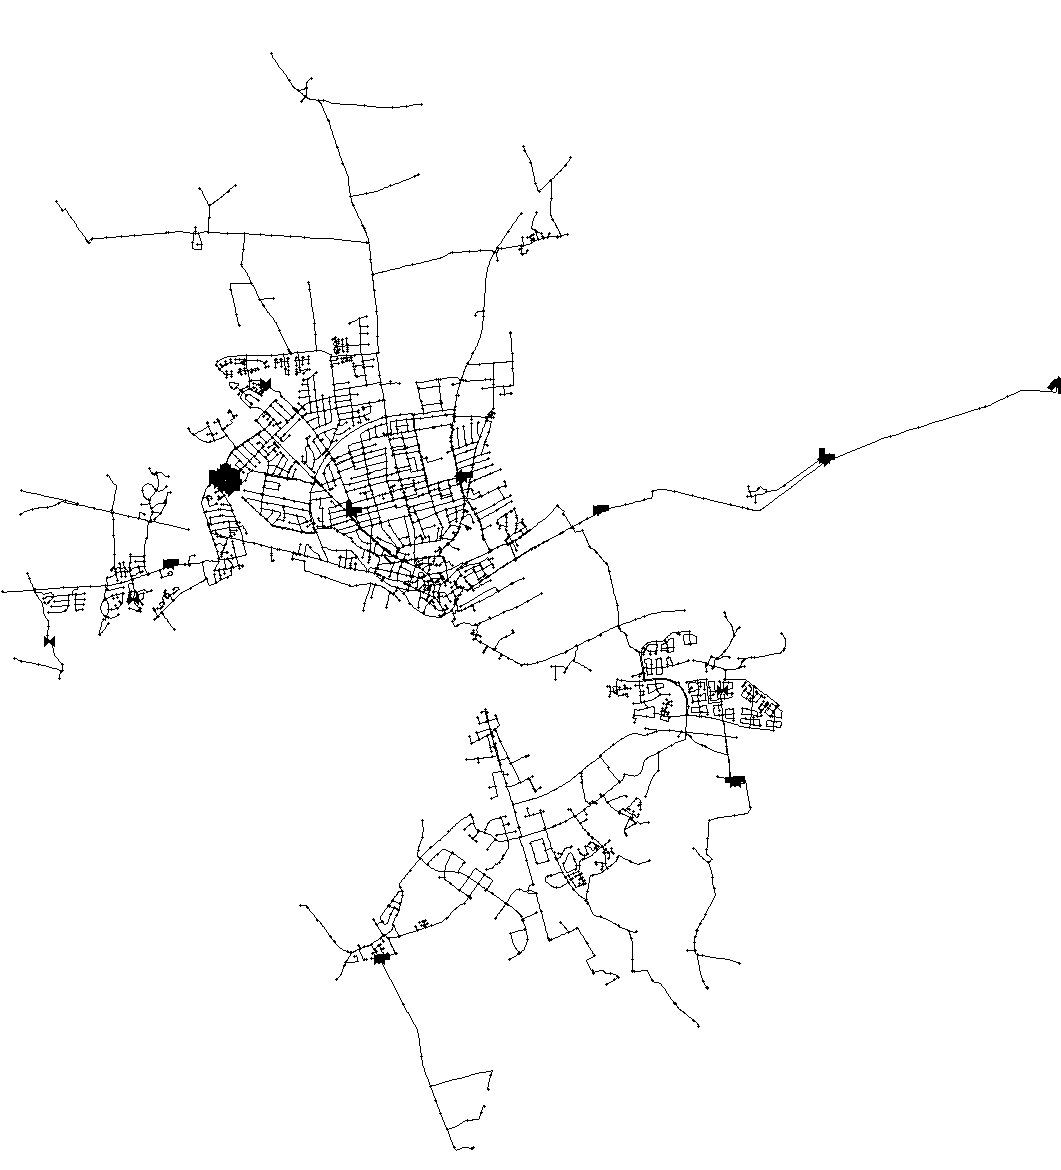
\includegraphics[width=1\textwidth]{report/pictures/verdo_pic}
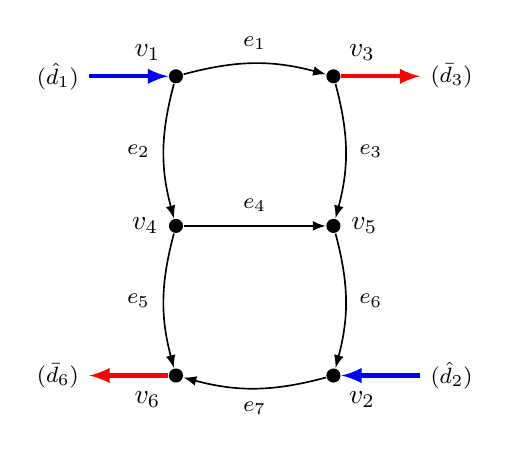
\begin{tikzpicture}[-latex ,auto,semithick,state/.style ={ draw,shape=circle,scale=0.7}]

\node[circle,fill,inner sep=1.8pt,label=above left: $v_1$] (A) at (0,0) {};
\node[circle,fill,inner sep=1.8pt,label=above right: $v_3$] (B) at (2,0) {};
\node[circle,fill,inner sep=1.8pt,label= left: $v_4$] (C) at (0,-1.9) {};
\node[circle,fill,inner sep=1.8pt,label= right: $v_5$] (D) at (2,-1.9) {};
\node[circle,fill,inner sep=1.8pt,label= below right: $v_2$] (E) at (2,-3.8) {};
\node[circle,fill,inner sep=1.8pt,label= below left: $v_6$] (F) at (0,-3.8) {};


\path (A) edge [bend right = -15] node[above  =0.05 cm] {\footnotesize$e_{1}$} (B);
\path (A) edge [bend right = 15] node[left  =0.05 cm] {\footnotesize$e_{2}$} (C);
\path (B) edge [bend right = -15] node[right  =0.05 cm] {\footnotesize$e_{3}$} (D);
\path (C) edge [bend right = 0] node[above  =0.05 cm] {\footnotesize$e_{4}$} (D);
\path (C) edge [bend right = 15] node[left  =0.05 cm] {\footnotesize$e_{5}$} (F);
\path (D) edge [bend right = -15] node[right  =0.05 cm] {\footnotesize$e_{6}$} (E);
\path (E) edge [bend right = -15] node[below  =0.05 cm] {\footnotesize$e_{7}$} (F);

\draw [-latex,line width=1.5pt,blue](-1.1,0) -- (-0.1,0);
\draw [-latex,line width=1.5pt,blue](3.1,-3.8) -- (2.1,-3.8);
\node at (-1.5,0) {\footnotesize $(\hat{d}_1)$};
\node at (3.5,-3.8) {\footnotesize $(\hat{d}_2)$};
\node at (3.5,0) {\footnotesize $(\bar{d}_3)$};
\node at (-1.5,-3.8) {\footnotesize $(\bar{d}_6)$};
\draw [-latex,line width=1.5pt,red](2.1,0) -- (3.1,0);
\draw [-latex,line width=1.5pt,red](-0.1,-3.8) -- (-1.1,-3.8);
\end{tikzpicture}
 
\caption{Graph of a simple multi-inlet network.}
\label{fig:example1_graph}
\end{figure}

In \figref{fig:example1_graph}, arrows illustrate the in-and outflows such that input flows are present in $v_1 $ and $v_2$, and user-consumption is defined only in $v_3$ and $v_6$. The diameters are the same for all pipes, however regarding the length, there are two types of pipes in this network. The corresponding parameters of the pipes, pumps, the elevation profile and the hourly demand variation is described in detail and can be found in (appref). 

The partitioning of edges in the network is chosen such that

\begin{equation}
  \label{edgeorientation_example1_T}
  \mathcal{E}_{\mathcal{T}} = \{ e_1, e_5, e_3, e_4 \} \equiv \{ e_{\mathcal{T},1}, e_{\mathcal{T},2}, e_{\mathcal{T},3}, e_{\mathcal{T},4}  \},
\end{equation}

and

\begin{equation}
\label{edgeorientation_example1_C}
  \mathcal{E}_\mathcal{C} = \{e_2, e_6, e_7\} \equiv \{e_{\mathcal{C},1}, e_{\mathcal{C},2}, e_{\mathcal{C},3}\},
\end{equation}.

The corresponding vectors describing the pressures and flows in vertices and edges, respectively, furthermore the elevation and distribution profiles are given such that

\begin{equation}
\label{example1_signals_constants}
p(t) =
 \begin{pmatrix} 
 \bar{p}_3(t) \\[1.3pt] 
 \bar{p}_4(t) \\[1.3pt]
 \bar{p}_5(t) \\[1.3pt] 
 \bar{p}_6(t) \\[1.3pt] 
 \hat{p}_1(t) \\[1.3pt] 
 \hat{p}_2(t) \\[1.3pt] 
 \end{pmatrix}
 , \hspace{5mm}
 d(t) =  \begin{pmatrix} 
 \bar{d}_3(t) \\[1pt] 
 0 \\[1pt]
 0 \\[1pt] 
 \bar{d}_6(t) \\[1pt] 
 \hat{d}_1(t) \\[1pt] 
 \hat{d}_2(t) \\[1pt] 
 \end{pmatrix}
 , \hspace{5mm}
 h =  \begin{pmatrix} 
 \bar{h}_3 \\[1pt] 
 \bar{h}_4 \\[1pt]
 \bar{h}_5 \\[1pt] 
 \bar{h}_6 \\[1pt] 
 0 \\[1pt] 
 0 \\[1pt] 
 \end{pmatrix}
 , \hspace{5mm}
 v =  \begin{pmatrix} 
 v_3 \\[1pt] 
 0 \\[1pt]
 0 \\[1pt] 
 v_6 \\[1pt]
 \end{pmatrix}.
\end{equation}

From this arrangement of the edges and nodes, it follows that the sub-matrix, $\bar{H}_{\mathcal{T}}$, which maps non-inlet vertices to edges in set $\mathcal{E}_{\mathcal{T}}$, is invertible. 

Since there are two nodes in the system with demand, the total flow leaving the network can be written as

\begin{equation}
  \label{consumption1}
  \sigma(t) = -\bar{d}_3(t) - \bar{d}_6(t).
\end{equation}

Having the input pressures and the parameters of the network, the output pressures, i.e. the pressures in the non-inlet vertices can be calculated. However, first recall \eqref{meshresult2}, 

\begin{equation}
  \label{ac_eq} 
  g(q_{\mathcal{C}}) = f_{\mathcal{C}}(q_\mathcal{C}) - A_1(\hat{p} + \hat{h}) + A_2 f_{\mathcal{T}}(A_3 q_\mathcal{C} + A_4 \bar{d}) = 0.
\end{equation}

\begin{minipage}[t]{0.4\textwidth}
where\\
\hspace*{8mm} $A_1 = \hat{H}^T_{\mathcal{C}} -\bar{H}^T_{\mathcal{C}}\bar{H}^{-T}_{\mathcal{T}}\hat{H}^T_{\mathcal{T}}$, \vspace*{1.5mm}  \\
\hspace*{8mm} $A_2 = -\bar{H}^T_{\mathcal{C}}\bar{H}^{-T}_{\mathcal{T}}$, \vspace*{1.5mm}  \\
\hspace*{8mm} $A_3 = -\bar{H}^{-1}_{\mathcal{T}} \bar{H}_{\mathcal{C}} $, \vspace*{1.5mm}\\
\hspace*{8mm} $A_4 = \bar{H}^{-1}_{\mathcal{T}}$. 
\end{minipage}

On account of non-linearity in \eqref{ac_eq},  it is not possible to solve the network analysis problem analytically. Instead, iterative numerical solution methods are used. As $g(q_{\mathcal{C}})$ is differentiable with respect to $q_{\mathcal{C}}$, gradient-based root finding algorithms such as Newton-Raphson method can be used. With iterative methods, initial values of flows are repeatedly adjusted until the difference between two successive iterates is within an acceptable tolerance.  Furthermore, we know from the homogeneity and monotonicity property of $g(q_{\mathcal{C}})$ that the function is a homeomorphism in $q_{\mathcal{C}}$, therefore its root is unique. Using gradient-based searching methods, and squaring $g(q_{\mathcal{C}})$ 

\begin{equation}
\label{gradient_search} 
  2 \frac{\partial g^T(q_{\mathcal{C}})}{\partial q_{\mathcal{C}}} g(q_{\mathcal{C}}) = 0, 
\end{equation}

the unique solution can be found. Furthermore, if $g^T(q_{\mathcal{C}}) g(q_{\mathcal{C}})$ is convex, the solution is the global minimum. By solving \eqref{ac_eq} for $a_{\mathcal{C}}$, the non-inlet pressures and all flows in the network can be calculated in terms of the input pressures and the total demand in the network. In order to obtain these values, the previously-derived output equation in \eqref{model_multiinlet1} can be used. 

In the simulation, the most simple case is considered, when the total flow demand in the network varies, however the distribution among vertices remains the same. In this case, $v$ is a constant vector, and the base demands in all vertices are the same. 

The variation curve for the input pressures are set the same in both EPANET and in the simulator. 

\begin{figure}[H]
\centering
\begin{subfigure}{.49\textwidth}
\centering
  % This file was created by matlab2tikz.
%
%The latest updates can be retrieved from
%  http://www.mathworks.com/matlabcentral/fileexchange/22022-matlab2tikz-matlab2tikz
%where you can also make suggestions and rate matlab2tikz.
%
\definecolor{mycolor1}{rgb}{0.00000,0.44700,0.74100}%
\definecolor{mycolor2}{rgb}{0.85000,0.32500,0.09800}%
%
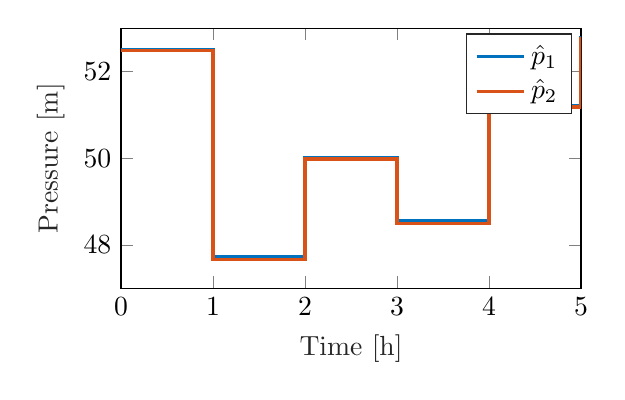
\begin{tikzpicture}

\begin{axis}[%
width=2.3in,
height=1.3in,
at={(0.766in,0.474in)},
scale only axis,
xmin=0,
xmax=5,
xlabel style={font=\color{white!15!black}},
xlabel={Time [h]},
ymin=47,
ymax=53,
ylabel style={font=\color{white!15!black}},
ylabel={Pressure [m]},
axis background/.style={fill=white},
%title style={font=\bfseries},
%title={Inlet pressures},
%xmajorgrids,
%ymajorgrids,
legend style={legend cell align=left, align=left, draw=white!15!black}
]
\addplot[const plot, color=mycolor1, line width=1.2pt] table[row sep=crcr] {%
0	52.51\\
1	47.74\\
2	50.02\\
3	48.57\\
4	51.22\\
5	52.81\\
};
\addlegendentry{$\hat{p}_1$}

\addplot[const plot, color=mycolor2, line width=1.2pt] table[row sep=crcr] {%
0	52.49\\
1	47.66\\
2	49.98\\
3	48.5\\
4	51.18\\
5	52.8\\
};
\addlegendentry{$\hat{p}_2$}

\end{axis}
\end{tikzpicture}% 
  \caption{Inlet pressures, $(\hat{p})$}
  \label{fig:sub11_example1}
\end{subfigure}
\begin{subfigure}{.49\textwidth}
\centering
  % This file was created by matlab2tikz.
%
%The latest updates can be retrieved from
%  http://www.mathworks.com/matlabcentral/fileexchange/22022-matlab2tikz-matlab2tikz
%where you can also make suggestions and rate matlab2tikz.
%
\definecolor{mycolor1}{rgb}{0.00000,0.44700,0.74100}%
\definecolor{mycolor2}{rgb}{0.85000,0.32500,0.09800}%
%
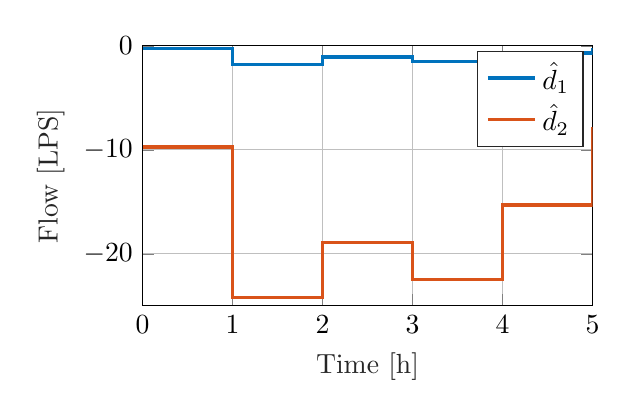
\begin{tikzpicture}

\begin{axis}[%
width=2.25in,
height=1.3in,
at={(0.791in,0.461in)},
scale only axis,
xmin=0,
xmax=5,
xlabel style={font=\color{white!15!black}},
xlabel={Time [h]},
ymin=-25,
ymax=0,
ylabel style={font=\color{white!15!black}},
ylabel={Flow [LPS]},
axis background/.style={fill=white},
%title style={font=\bfseries},
%title={Inlet demands},
xmajorgrids,
ymajorgrids,
legend style={legend cell align=left, align=left, draw=white!15!black}
]
\addplot[const plot, color=mycolor1, line width=1.2pt] table[row sep=crcr] {%
0	-0.27002029288415\\
1	-1.78959208760883\\
2	-1.07885170290758\\
3	-1.53102470893297\\
4	-0.688152757407579\\
5	-0.175509754602786\\
};
\addlegendentry{$\hat{d}_1$}

\addplot[const plot, color=mycolor2, line width=1.2pt] table[row sep=crcr] {%
0	-9.72997970711585\\
1	-24.2104079123912\\
2	-18.9211482970924\\
3	-22.468975291067\\
4	-15.3118472425924\\
5	-7.82449024539721\\
};
\addlegendentry{$\hat{d}_2$}

\end{axis}
\end{tikzpicture}% 
  \caption{Inlet demands, $(\hat{d})$}
  \label{fig:sub22_example1}
\end{subfigure}
\caption{Signals describing the input pressures(left) and flows(right) of the pumping stations.}
\label{fig:inlet_pressures_demands}
\end{figure}

\begin{figure}[H]
\centering
\begin{subfigure}{.49\textwidth}
\centering
  % This file was created by matlab2tikz.
%
%The latest updates can be retrieved from
%  http://www.mathworks.com/matlabcentral/fileexchange/22022-matlab2tikz-matlab2tikz
%where you can also make suggestions and rate matlab2tikz.
%
\definecolor{mycolor1}{rgb}{0.00000,0.44700,0.74100}%
\definecolor{mycolor2}{rgb}{0.85000,0.32500,0.09800}%
%
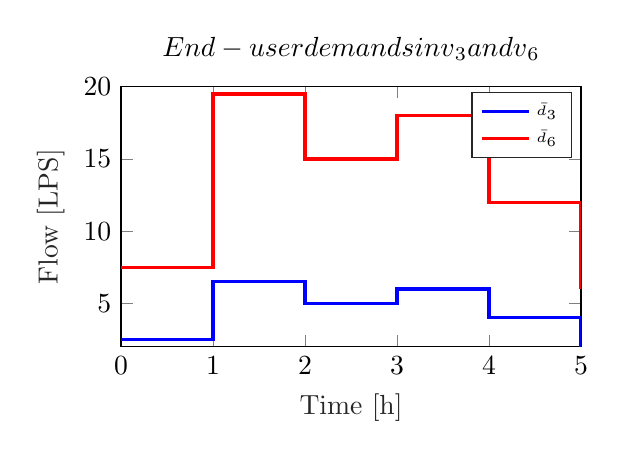
\begin{tikzpicture}

\begin{axis}[%
width=2.3in,
height=1.3in,
at={(0.758in,0.481in)},
scale only axis,
xmin=0,
xmax=5,
xlabel style={font=\color{white!15!black}},
xlabel={Time [h]},
ymin=2,
ymax=20,
ylabel style={font=\color{white!15!black}},
ylabel={Flow [LPS]},
axis background/.style={fill=white},
title style={},
title={$\text{End-user demands in v}_\text{3}\text{ and v}_\text{6}$},
%xmajorgrids,
%ymajorgrids,
legend style={legend cell align=left, align=left, draw=white!15!black}
]
\addplot[const plot, color=blue, line width=1.2pt] table[row sep=crcr] {%
0	2.5\\
1	6.5\\
2	5\\
3	6\\
4	4\\
5	2\\
};
\addlegendentry{\tiny $\bar{d}_3$}

\addplot[const plot, color=red, line width=1.2pt] table[row sep=crcr] {%
0	7.5\\
1	19.5\\
2	15\\
3	18\\
4	12\\
5	6\\
};
\addlegendentry{\tiny $\bar{d}_6$}

\end{axis}
\end{tikzpicture}% 
  \caption{Non-inlet demands, $(\bar{d})$}
  \label{fig:sub21_example1}
\end{subfigure}
\begin{subfigure}{.49\textwidth}
\centering
  % This file was created by matlab2tikz.
%
%The latest updates can be retrieved from
%  http://www.mathworks.com/matlabcentral/fileexchange/22022-matlab2tikz-matlab2tikz
%where you can also make suggestions and rate matlab2tikz.
%
\definecolor{mycolor1}{rgb}{0.00000,0.44700,0.74100}%
\definecolor{mycolor2}{rgb}{0.85000,0.32500,0.09800}%
\definecolor{mycolor3}{rgb}{0.92900,0.69400,0.12500}%
\definecolor{mycolor4}{rgb}{0.49400,0.18400,0.55600}%
%
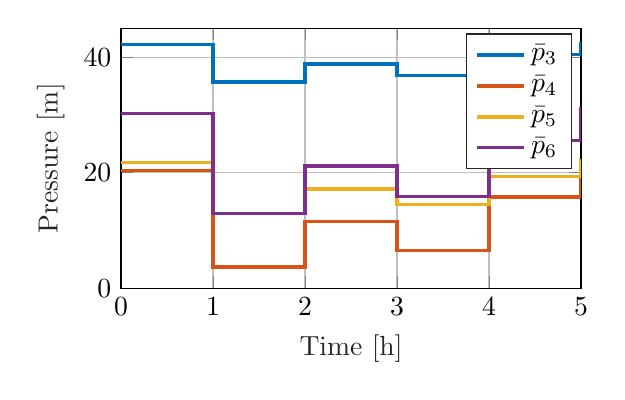
\begin{tikzpicture}

\begin{axis}[%
width=2.3in,
height=1.3in,
at={(0.758in,0.481in)},
scale only axis,
xmin=0,
xmax=5,
xlabel style={font=\color{white!15!black}},
xlabel={Time [h]},
ymin=0,
ymax=45,
ylabel style={font=\color{white!15!black}},
ylabel={Pressure [m]},
axis background/.style={fill=white},
%title style={font=\bfseries},
%title={Non-inlet pressures $(\bar{p})$},
xmajorgrids,
ymajorgrids,
legend style={legend cell align=left, align=left, draw=white!15!black}
]
\addplot[const plot, color=mycolor1, line width=1.2pt] table[row sep=crcr] {%
0	42.21\\
1	35.712\\
2	38.82\\
3	36.842\\
4	40.452\\
5	42.618\\
};
\addlegendentry{$\bar{p}_3$}

\addplot[const plot, color=mycolor2, line width=1.2pt] table[row sep=crcr] {%
0	20.3672640689439\\
1	3.67476567889016\\
2	11.6071871859654\\
3	6.54234407877965\\
4	15.7956885662872\\
5	21.4335225222452\\
};
\addlegendentry{$\bar{p}_4$}

\addplot[const plot, color=mycolor3, line width=1.2pt] table[row sep=crcr] {%
0	21.7881086237316\\
1	12.9652322870728\\
2	17.1730521589117\\
3	14.4909102062663\\
4	19.3873080072803\\
5	22.3468148852399\\
};
\addlegendentry{$\bar{p}_5$}

\addplot[const plot, color=mycolor4, line width=1.2pt] table[row sep=crcr] {%
0	30.2597113346647\\
1	12.9533643088574\\
2	21.1795244882205\\
3	15.9271407367542\\
4	25.5211869947594\\
5	31.3646680673769\\
};
\addlegendentry{$\bar{p}_6$}

\end{axis}
\end{tikzpicture}% 
  \caption{Non-inlet pressures, $(\bar{p})$}
  \label{fig:sub22_example1}
\end{subfigure}
\caption{Signals describing the demand flows by the end-users(left) and output pressures(right) in the network.}
\label{fig:noninlet_demands_noninlet_pressures}
\end{figure}

\begin{figure}[H]
\centering
\begin{subfigure}{.49\textwidth}
\centering
  % This file was created by matlab2tikz.
%
%The latest updates can be retrieved from
%  http://www.mathworks.com/matlabcentral/fileexchange/22022-matlab2tikz-matlab2tikz
%where you can also make suggestions and rate matlab2tikz.
%
\definecolor{mycolor1}{rgb}{0.00000,0.44700,0.74100}%
\definecolor{mycolor2}{rgb}{0.85000,0.32500,0.09800}%
\definecolor{mycolor3}{rgb}{0.92900,0.69400,0.12500}%
%
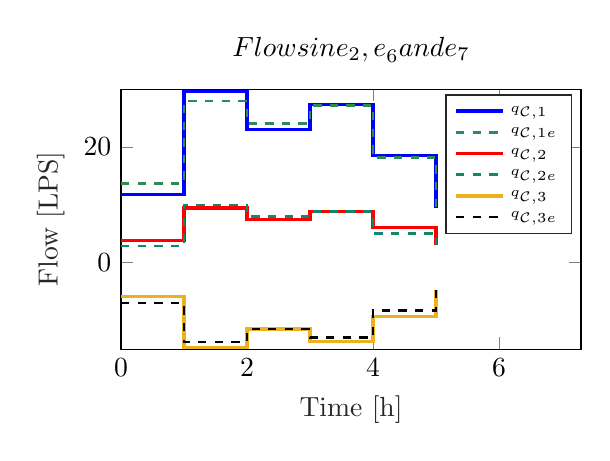
\begin{tikzpicture}

\begin{axis}[%
width=2.3in,
height=1.3in,
at={(0.758in,0.481in)},
scale only axis,
xmin=0,
xmax=7.3,
xlabel style={font=\color{white!15!black}},
xlabel={Time [h]},
ymin=-15,
ymax=30,
ylabel style={font=\color{white!15!black}},
ylabel={Flow [LPS]},
axis background/.style={fill=white},
title style={},
title={$\text{Flows in e}_\text{2}\text{, e}_\text{6}\text{ and e}_\text{7}$},
%xmajorgrids,
%ymajorgrids,
legend style={legend cell align=left, align=left, draw=white!15!black}
]
\addplot[const plot, color=blue, line width=1.2pt] table[row sep=crcr] {%
0	11.7502570959187\\
1	29.5561012463149\\
2	23.0126657096865\\
3	27.3936960334265\\
4	18.5662622910719\\
5	9.43871589453002\\
};
\addlegendentry{\tiny $q_{\mathcal{C},1}$}

\addplot[const plot, dashed, color=SeaGreen, line width=1pt] table[row sep=crcr] {%
0	13.7502570959187\\
1	27.9561012463149\\
2	24.0126657096865\\
3	27.1936960334265\\
4	18.1662622910719\\
5	8.43871589453002\\
};
\addlegendentry{\tiny $q_{\mathcal{C},1e}$}

\addplot[const plot, color=red, line width=1.2pt] table[row sep=crcr] {%
0	3.85877138476544\\
1	9.45870515475531\\
2	7.4303780100986\\
3	8.79458158128527\\
4	6.03871892954993\\
5	3.10763052781182\\
};
\addlegendentry{\tiny $q_{\mathcal{C},2}$}

\addplot[const plot, dashed, color=PineGreen, line width=1pt] table[row sep=crcr] {%
0	2.85877138476544\\
1	9.95870515475531\\
2	7.99303780100986\\
3	8.79458158128527\\
4	5.03871892954993\\
5	3.10763052781182\\
};
\addlegendentry{\tiny $q_{\mathcal{C},2e}$}

\addplot[const plot, color=mycolor3, line width=1.2pt] table[row sep=crcr] {%
0	-5.87120832235041\\
1	-14.7517027576359\\
2	-11.4907702869938\\
3	-13.6743937097818\\
4	-9.27312831304249\\
5	-4.71685971758539\\
};
\addlegendentry{\tiny $q_{\mathcal{C},3}$}

\addplot[const plot, dashed, color=black, line width=1pt] table[row sep=crcr] {%
0	-6.99120832235041\\
1	-13.7517027576359\\
2	-11.4907702869938\\
3	-12.9743937097818\\
4	-8.27312831304249\\
5	-4.71685971758539\\
};
\addlegendentry{\tiny $q_{\mathcal{C},3e}$}

\end{axis}
\end{tikzpicture}% 
  \caption{Flows in $\mathcal{C}$, $(q_{\mathcal{C}})$}
  \label{fig:sub31_example1}
\end{subfigure}
\begin{subfigure}{.49\textwidth}
\centering
  % This file was created by matlab2tikz.
%
%The latest updates can be retrieved from
%  http://www.mathworks.com/matlabcentral/fileexchange/22022-matlab2tikz-matlab2tikz
%where you can also make suggestions and rate matlab2tikz.
%
\definecolor{mycolor1}{rgb}{0.00000,0.44700,0.74100}%
\definecolor{mycolor2}{rgb}{0.85000,0.32500,0.09800}%
\definecolor{mycolor3}{rgb}{0.92900,0.69400,0.12500}%
\definecolor{mycolor4}{rgb}{0.49400,0.18400,0.55600}%
%
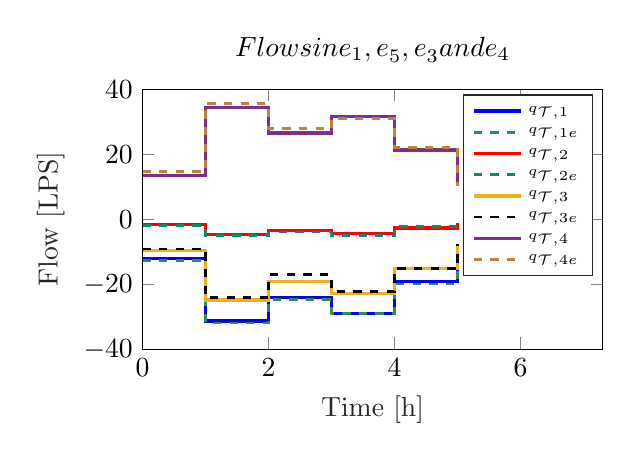
\begin{tikzpicture}

\begin{axis}[%
width=2.3in,
height=1.3in,
at={(0.758in,0.481in)},
scale only axis,
xmin=0,
xmax=7.3,
xlabel style={font=\color{white!15!black}},
xlabel={Time [h]},
ymin=-40,
ymax=40,
ylabel style={font=\color{white!15!black}},
ylabel={Flow [LPS]},
axis background/.style={fill=white},
title style={},
title={$\text{Flows in e}_\text{1}\text{, e}_\text{5}\text{, e}_\text{3}\text{ and e}_\text{4}$},
%xmajorgrids,
%ymajorgrids,
legend style={legend cell align=left, align=left, draw=white!15!black}
]
\addplot[const plot, color=blue, line width=1.2pt] table[row sep=crcr] {%
0	-12.0202773888028\\
1	-31.3456933339238\\
2	-24.0915174125941\\
3	-28.9247207423594\\
4	-19.2544150484795\\
5	-9.61422564913281\\
};
\addlegendentry{\tiny $q_{\mathcal{T},1}$}

\addplot[const plot, dashed, color=SeaGreen, line width=1pt] table[row sep=crcr] {%
0	-12.7202773888028\\
1	-31.9456933339238\\
2	-24.7915174125941\\
3	-28.9247207423594\\
4	-19.9544150484795\\
5	-9.61422564913281\\
};
\addlegendentry{\tiny $q_{\mathcal{T},1e}$}

\addplot[const plot, color=red, line width=1.2pt] table[row sep=crcr] {%
0	-1.62879167764959\\
1	-4.74829724236414\\
2	-3.50922971300619\\
3	-4.32560629021824\\
4	-2.72687168695751\\
5	-1.28314028241461\\
};
\addlegendentry{\tiny $q_{\mathcal{T},2}$}

\addplot[const plot, dashed, color=PineGreen, line width=1pt] table[row sep=crcr] {%
0	-1.92879167764959\\
1	-4.94829724236414\\
2	-3.90922971300619\\
3	-4.92560629021824\\
4	-2.12687168695751\\
5	-1.28314028241461\\
};
\addlegendentry{\tiny $q_{\mathcal{T},2e}$}

\addplot[const plot, color=mycolor3, line width=1.2pt] table[row sep=crcr] {%
0	-9.52027738880282\\
1	-24.8456933339238\\
2	-19.0915174125941\\
3	-22.9247207423594\\
4	-15.2544150484795\\
5	-7.6142256491328\\
};
\addlegendentry{\tiny $q_{\mathcal{T},3}$}

\addplot[const plot, dashed, color=black, line width=1pt] table[row sep=crcr] {%
0	-9.12027738880282\\
1	-24.1456933339238\\
2	-17.0915174125941\\
3	-22.1247207423594\\
4	-15.2544150484795\\
5	-7.6142256491328\\
};
\addlegendentry{\tiny $q_{\mathcal{T},3e}$}

\addplot[const plot, color=mycolor4, line width=1.2pt] table[row sep=crcr] {%
0	13.3790487735683\\
1	34.3043984886791\\
2	26.5218954226927\\
3	31.7193023236447\\
4	21.2931339780294\\
5	10.7218561769446\\
};
\addlegendentry{\tiny $q_{\mathcal{T},4}$}

\addplot[const plot, dashed, color=brown, line width=1pt] table[row sep=crcr] {%
0	14.5790487735683\\
1	35.5043984886791\\
2	27.9218954226927\\
3	31.1193023236447\\
4	21.9931339780294\\
5	10.1218561769446\\
};
\addlegendentry{\tiny $q_{\mathcal{T},4e}$}


\end{axis}
\end{tikzpicture}% 
  \caption{Flows in $\mathcal{T}$, $(q_{\mathcal{T}})$}
  \label{fig:sub31_example1}
\end{subfigure}
\caption{Signals describing the flows in all pipes in the network.}
\label{fig:flows_C_T}
\end{figure}

\newpage

\section{Inclusion of elevated reservoirs}
\label{inclusion_of_reservoirs}

When a WT is being attached to an existing pipe network, certain properties of the previous system must be modified. Regarding the underlying graph of the network, when a WT is attached, the vertex to which the tank is connected becomes a vertex with a demand. However, the demand flow which describes the filling and emptying process of the tank, in this case, is not directly related to any user consumption profile, since flow can go into and come out of the tank. Therefore, the constraint on demand flows, described in \eqref{non_inlet_constraint} is not true in case of elevated reservoirs, as the demand can be both positive or negative. For this reason, demands on the reservoirs are treated as inputs and added to the nodes marked with hats $\hat{p}$ and $\hat{d}$. The nodes on which demand of elevated reservoirs are defined are partitioned from the input flows of the pumps such that 

\begin{subequations}
\begin{equation}
\label{tank_inclusion_separation_of_input_demand}
\hat{d} = F \hat{d}_t + G \hat{d}_c ,
\end{equation}


 \begin{minipage}[t]{0.20\textwidth}
where\\
\hspace*{8mm} $\hat{d}_t \in \: \mathbb{R}^{(l \times 1)}$\\
\hspace*{8mm} $\hat{d}_c \in \: \mathbb{R}^{(c \times 1\!)}$ \\
\newline
\hspace*{6mm} $F^T \in \: \mathbb{R}^{(l\! \times \!c\!+\!l)}$ \\
\hspace*{6mm} $G^T \in \: \mathbb{R}^{(c\! \times \!c\!+\!l )}$
\end{minipage}
\begin{minipage}[t]{0.68\textwidth}
\vspace*{2mm}
is the vector including the nodal demands of the tanks,\\
is the the vector including the nodal demands of the pump inputs, \\
is a mapping which selects the nodes belonging to tanks, \\
is a mapping which selects the nodes belonging to pump inputs.
\end{minipage}

The same partitioning is done for the input pressures and elevation, regarding pumps and tanks

\begin{equation}
\label{tank_inclusion_separation_of_input_pressure_elevation1}
\hat{h} = F \hat{h}_t + G \hat{h}_c, 
\end{equation}

\begin{equation}
\label{tank_inclusion_separation_of_input_pressure_elevation2}
\hat{p} = F \hat{p}_t + G \hat{p}_c,
\end{equation}

\end{subequations}

 \begin{minipage}[t]{0.20\textwidth}
where\\
\hspace*{8mm} $\hat{h}_t \in \: \mathbb{R}^{(l \times 1)}$\\
\hspace*{8mm} $\hat{h}_c \in \: \mathbb{R}^{(c  \times  1)}$ \\
\newline
\hspace*{8mm} $\hat{p}_t \in \: \mathbb{R}^{(l \times 1)}$\\
\hspace*{8mm} $\hat{p}_c \in \: \mathbb{R}^{(c \times 1)}$ 
\end{minipage}
\begin{minipage}[t]{0.68\textwidth}
\vspace*{2mm}
is the vector including the elevation of the tanks,\\
is the the vector including the elevation of the pump stations,\\
is the vector including the absolute pressures in the tanks,\\
is the the vector including the absolute pressures of the pump inputs.
\end{minipage}

With the inclusion of tanks, the network is not only constrained by the static pressure and flow relation, as in case of the model without tanks, but also governed by the dynamic equation describing the WT. These dynamics act as integrators on the flows which go in or out of the tank, $\hat{d}_t$. In terms of $\hat{d}_t$, the dynamics of the tanks set the pressure contribution, $\hat{p}_t$ , as an input to the distribution system. The block diagram of such system is shown in \figref{fig:WT_system_blockdiagram}.

%Pumping stations and waterworks in Randers
\begin{figure}[H]
\centering
%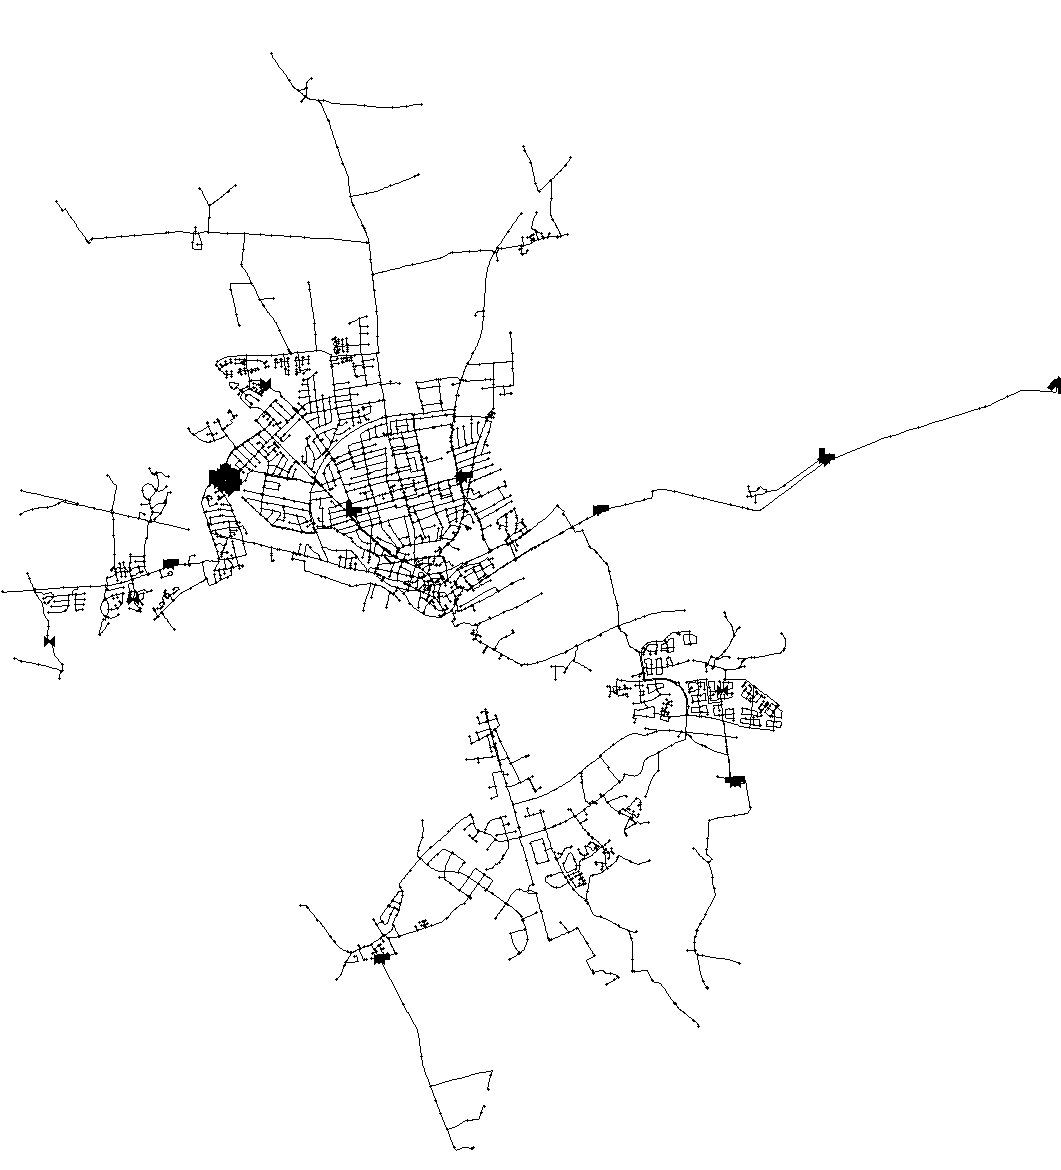
\includegraphics[width=1\textwidth]{report/pictures/verdo_pic}
 \usetikzlibrary{arrows}
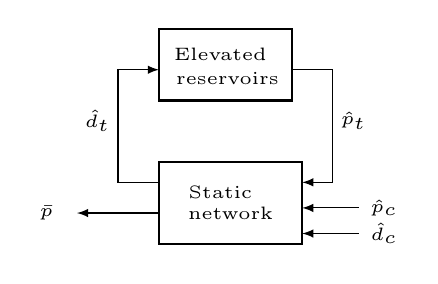
\begin{tikzpicture}[scale=1.3,transform shape]

\node at (-1.2,-2.5) {\tiny Static};
\node at (-1.1,-2.7) {\tiny network};
\node at (-1.2,-1.15) {\tiny Elevated};
\node at (-1.13,-1.38) {\tiny reservoirs};
\node at (0.1,-1.8) {\tiny $\hat{p}_t$};
\node at (-2.4,-1.8) {\tiny $\hat{d}_t$};
\node at (0.4,-2.65) {\tiny $\hat{p}_c$};
\node at (0.4,-2.9) {\tiny $\hat{d}_c$};
\node at (-2.9,-2.7) {\tiny $\bar{p}$};

\draw [thick] (-1.8,-0.9) rectangle (-0.5,-1.6);
\draw [thick] (-1.8,-2.2) rectangle (-0.4,-3);
\draw [-latex](-0.5,-1.3) -- (-0.1,-1.3) -- (-0.1,-2.4) -- (-0.4,-2.4);
\draw [-latex](0.15,-2.65) -- (-0.4,-2.65);
\draw [-latex](0.15,-2.9) -- (-0.4,-2.9);
\draw [-latex](-1.8,-2.4) -- (-2.2,-2.4) -- (-2.2,-1.3) -- (-1.8,-1.3);
\draw [-latex](-1.8,-2.7) -- (-2.6,-2.7);
\end{tikzpicture} 
\caption{Block diagram of the system with WTs.}
\label{fig:WT_system_blockdiagram}
\end{figure}

where the 'Elevated reservoirs' block represents the subsystem with dynamics, and the 'Static network' subsystem is governed by the algebraic flow and pressure relations which describe the pipe network. 

When elevated reservoirs are introduced in the network, the system usually operates such that the control inputs are the flows, $\hat{d}$, as this is the most practical and robust way to control the network. In fact, this is the case regarding the Randers WSS, as the two pumping stations which are filling up the tanks are controlled by flow, as it was explained in \secref{waterworks_and_pumping_stations}. 

This modelling approach is different, however,  from what is handled in case of a network without a tank, since instead of using the pressures, $\hat{p}$, the inlet flows, $\hat{d_c}$, are considered as inputs. Furthermore, regarding the dynamics, the filling and emptying of a tank is dependent on how much flow is delivered by the pumps. This inlet flow is provided by multiple pumping stations, however, a distinction has to be made between the presence of single or multiple WTs in the network. In the former case, the flows delivered by the pumps are filling or emptying the one and only tank in the network. In the latter case, however, the model needs to be able to handle the flow distribution among the different WTs, meaning that different pumping stations can have different filling or emptying effects on the different WTs. Therefore, in the following, the two different approaches are presented. 


\section{Multi-inlet, single-WT model}
\label{multi_inlet_single_WT_model}

Recalling the dynamic equation of one tank, in \eqref{wt_model2}

\begin{equation}
\label{wt_model_demand1}
\dot{\hat{p}}_{t} = -\tau \hat{d}_{t},
\end{equation}

it is seen that the flow, $\hat{d}_t$, needs to be expressed in terms of the inputs, $\hat{d}_c$. In order to express the demand regarding a tank, the whole network is treated as one node, as illustrated in \figref{fig:onenode_system}. 

 %Network illustration as one node
\begin{figure}[H]
\centering
%
\includegraphics[width=0.35\textwidth]{report/pictures/missingfigure}
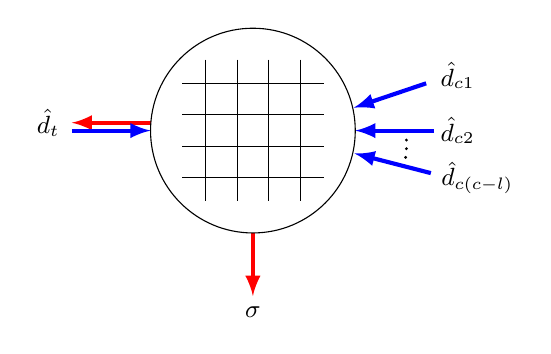
\begin{tikzpicture}[scale=1,transform shape]

\draw [-latex,line width=1.5pt,red](-0.3,-1.9) -- (-0.3,-2.7);
\draw [-latex,line width=1.5pt,blue](2,-0.6) -- (1,-0.6);
\draw [-latex,line width=1.5pt,blue](1.9,0) -- (0.98,-0.31);
\draw [-latex,line width=1.5pt,red](-1.6,-0.5) -- (-2.6,-0.5);
\draw [-latex,line width=1.5pt,blue](-2.6,-0.6) -- (-1.6,-0.6);
\draw [-latex,line width=1.5pt,blue](1.96,-1.14) -- (0.99,-0.89);

\draw (-0.9,0.3) -- (-0.9,-1.5);
\draw (-0.5,0.3) -- (-0.5,-1.5);
\draw (-0.1,0.3) -- (-0.1,-1.5);
\draw (0.3,0.3) -- (0.3,-1.5);
\draw (-1.2,0) -- (0.6,0);
\draw (-1.2,-0.4) -- (0.6,-0.4);
\draw (-1.2,-0.8) -- (0.6,-0.8);
\draw (-1.2,-1.2) -- (0.6,-1.2);
\draw  (-0.3,-0.6) ellipse (1.3 and 1.3);

\node at (2.3,0.1) {\small $\hat{d}_{c1}$};
\node at (2.3,-0.6) {\small $\hat{d}_{c2}$};
\node at (2.55,-1.2) {\small $\hat{d}_{c(c-l)}$};
\node at (-2.9,-0.5) {\small $\hat{d}_t$};
\node at (-0.3,-2.9) {\small $\sigma$};

\node[circle,fill,inner sep=0.4pt] (A) at (1.65,-0.72) {};
\node[circle,fill,inner sep=0.4pt] (A) at (1.64,-0.94) {};
\node[circle,fill,inner sep=0.4pt] (A) at (1.65,-0.83) {};

\end{tikzpicture} 
\caption{Mass balance on the network with one WT.}
\label{fig:onenode_system}
\end{figure}

According to the mass-balance in the network, and using the corresponding partitioning as shown in \figref{fig:onenode_system}, the balance equation on all demand flows can be written in the form of

\begin{equation}
\label{massbalance_model2}
1^Td 
 =
 1^T
\begin{pmatrix} 
\bar{d} \\
\hat{d}
\end{pmatrix}
=
1^T
\begin{pmatrix} 
-v \sigma \\
\hat{d}_c \\
\hat{d}_t 
\end{pmatrix}
=
0
\end{equation}

Now, expressing $\hat{d}_t $ from \eqref{massbalance_model2} yields

\begin{equation}
\label{massbalance_model2_1}
\hat{d}_t  = \sigma - 1^T \hat{d}_c,
\end{equation}

where it is shown, that if the control flows, $\hat{d}_c$, are higher than the total non-inlet demand, $\sigma$, the tank is being filled, and the tank is emptied if $\hat{d}_c$ is lower than $\sigma$. Thus, the system dynamics can be reformulated such that

\begin{equation}
\label{wt_model_demandd}
\dot{\hat{p}}_t = -\tau (\sigma - 1^T \hat{d}_c).
\end{equation}

It is important to point out that this first order differential equation in \eqref{wt_model_demandd}, describes the mass-balance model of a single tank system, where the input flows equal to the overall demand in the network and the rate of change in storage in the tank. The result is not surprising, since according to \eqref{wt_model_demandd}, the water level, or pressure, fluctuates according to the in- and outflow of water, which relates to the pumping effort and demand in the network. 

In the single-WT modelling case, the dynamics can be described by a one-state, scalar equation, however the model is restricted to only one WT. As shown before, we know that this is not the case in the Randers WSS. Therefore, a more general description of the network is required, without restriction on the number of elevated reservoirs. 


\section{Multi-inlet, multi-WT model}
\label{multi_inlet_multi_WT_model}

In case when there are more than one WTs, the mass-balance equation, proposed in \eqref{massbalance_model2} is not applicable due to the fact that the pressures delivered by the tanks have to be balanced, similarly as in a simple connected-volume system. Therefore, a model framework is required which can handle the dynamics of multiple tanks, constrained by the static network and driven by the input flows of the pumping stations. In order to derive such model, the partitioning of the network is reconsidered. As described previously, the incidence matrix is partitioned such that 

\begin{equation}
\label{H_matrix_sub1}
H=
\begin{pmatrix}
\bar{H}_{\mathcal{T}} & \bar{H}_{\mathcal{C}} \\[3pt]
\hat{H}_{\mathcal{T}} & \hat{H}_{\mathcal{C}}
\end{pmatrix},
\end{equation}

where $\bar{H}_{\mathcal{T}}$ is invertible. This partitioning rule on the edges is kept, however in the following model description let us slightly modify the notation and partitioning of the vertices. Now let

\begin{equation}
  \label{vertices1_1}
  \mathcal{V} = \{\bar{\mathcal{V}}, \hat{\mathcal{V}} \}, 
\end{equation}

\begin{minipage}[t]{0.3\textwidth}
where\\
\hspace*{8mm} $\hat{\mathcal{V}} = \{\hat{v}_1, ..., \hat{v}_l\}$\\
\newline
and \\
\hspace*{8mm} $\bar{\mathcal{V}} = \{\bar{v}_1, ..., \bar{v}_{n-l}\}$ 
\end{minipage}
\begin{minipage}[t]{0.67\textwidth}
\vspace*{2mm}
 represents the vertices corresponding to the points where elevated reservoirs are connected,\\
 \newline
 represents the remaining vertices in the graph.
\end{minipage}

We originally defined $\bar{d}$ to describe non-inlet demands in the network and $\hat{d}$ to describe inlet-flows of the pumping stations, along with the demands of the WTs. With the redefined notation and partitioning of vertices, now we make sure that the vertices related to tanks are separated and all other points in the network are in the same set. So now, $\hat{d}$ describes flows regarding the WTs. In order to express the controlled inlet and non-inlet points in the network, the vectors related to the nodes marked with bars, $\bar{p}$ and $\bar{d}$, are split such that

\begin{subequations}

\begin{equation}
\label{barequation_sep1}
\bar{p} = K \bar{p}_{\mathcal{K}} + D \bar{p}_{\mathcal{D}}, 
\end{equation}

\begin{equation}
\label{barequation_sep2}
\bar{d} = K \bar{d}_{\mathcal{K}} + D \bar{d}_{\mathcal{D}},  
\end{equation}

\end{subequations}

 \begin{minipage}[t]{0.3\textwidth}
where\\
\hspace*{8mm} $\bar{p}_{\mathcal{K}}$ \\
\hspace*{8mm} $\bar{p}_{\mathcal{D}}$  \\
\hspace*{8mm} $\bar{d}_{\mathcal{K}}$ \\
\hspace*{8mm} $\bar{d}_{\mathcal{D}} = -v_{\mathcal{D}} \sigma$  \\
\hspace*{8mm} $K^T \in  \mathbb{R}^{(c  \times n-l)}$ \\
\newline
\hspace*{8mm} $D^T \in  \mathbb{R}^{(n-l-c  \times n-l)}$
\end{minipage}
\begin{minipage}[t]{0.68\textwidth}
\vspace*{2mm}
is the vector including the inlet pressures ,\\
is the the vector including the non-inlet pressures, \\
is the the vector including the controlled inlet flows, \\
is the the vector including the non-inlet demands, \\
is a mapping which selects the nodes belonging to the pumps, \\
is a mapping which selects the nodes belonging to the rest of the network except pumps and elevated reservoirs.
\end{minipage}

With this partitioning of the vertices, similarly to the model presented in \secref{multi_inlet_reduced_network_description}, Kirchhoff's and Ohm's law can be formulated. Recalling Kirchhoff's vertex law

\begin{equation}
\label{kirchhoffslaw_matrix}
H
 \begin{pmatrix} 
 q_\mathcal{T} \\[3pt]
 q_\mathcal{C} 
 \end{pmatrix}
 =
\begin{pmatrix} 
 \bar{d}  \\[3pt] 
 \hat{d}  
 \end{pmatrix},
\end{equation}

and recalling \eqref{ohmslaw_matrixform}, Ohm's law is given

\begin{equation}
\label{ohmslaw_matrixform}
 \begin{pmatrix} 
 f_{\mathcal{T}}(q_\mathcal{T}) \\[3pt]
 f_{\mathcal{C}}(q_\mathcal{C}) 
 \end{pmatrix}
 =
 \begin{pmatrix}
   \bar{H}^T_{\mathcal{T}} & \hat{H}^T_{\mathcal{T}} \\[3pt]
   \bar{H}^T_{\mathcal{C}} & \hat{H}^T_{\mathcal{C}} 
   \end{pmatrix}
   \begin{pmatrix} 
 \bar{p} + \bar{h} \\[3pt] 
 \hat{p} + \hat{h} 
 \end{pmatrix}.
\end{equation}

In order to get an expression for $\hat{d}$, describing the flows regarding the WTs, lets define matrix $\Omega$ as follows

\begin{equation}
\label{omega_matrix}
\Omega
=
\begin{pmatrix} 
 -\hat{H}_{\mathcal{T}}  \bar{H}^{-1}_{\mathcal{T}}  & I  
 \end{pmatrix}.
\end{equation}

Multiplying \eqref{kirchhoffslaw_matrix} with $\Omega$ from the left-hand side, $\hat{d}$ can be expressed in the form of

\begin{equation}
\label{WT_flows}
\hat{d} = (\hat{H}_{\mathcal{C}} - \hat{H}_{\mathcal{T}} \bar{H}^{-1}_{\mathcal{T}}\bar{H}_{\mathcal{C}})  q_\mathcal{C}  + \hat{H}_{\mathcal{T}} \bar{H}^{-1}_{\mathcal{T}} \bar{d}.
\end{equation}

As shown in \eqref{WT_flows}, the vertex law describes the dependencies of the WT demands on $\bar{d}$, which now consists of the pump inlet flows and the non-inlet demands in the rest of the network, and also shows the dependencies on $q_\mathcal{C}$. Recalling and rewriting the equation governing elevated reservoirs in matrix form, we can write the following

\begin{equation}
\label{WT_matrixform}
\Lambda \dot{\hat{p}} = - \hat{d},
\end{equation}

where $\Lambda = diag(\frac{1}{\tau_1},... ,\frac{1}{\tau_l}) \in \: \mathbb{R}^l_+$. 

Inserting $\hat{d}$ in \eqref{WT_flows}, into the WT dynamics leads to

\begin{equation}
\label{WT_matrixform_1}
\Lambda \dot{\hat{p}} = - (\hat{H}_{\mathcal{C}} - \hat{H}_{\mathcal{T}} \bar{H}^{-1}_{\mathcal{T}}\bar{H}_{\mathcal{C}})  q_\mathcal{C}  - \hat{H}_{\mathcal{T}} \bar{H}^{-1}_{\mathcal{T}} \bar{d}.
\end{equation}

Now, with the partitioning of $\bar{d}$, the inlet and non-inlet demands are inserted into \eqref{WT_matrixform_1}, resulting in the final governing expression of the dynamics

\begin{equation}
\label{WT_matrixform_final}
\Lambda \dot{\hat{p}} = - (\hat{H}_{\mathcal{C}} - \hat{H}_{\mathcal{T}} \bar{H}^{-1}_{\mathcal{T}}\bar{H}_{\mathcal{C}})  q_\mathcal{C}  - \hat{H}_{\mathcal{T}} \bar{H}^{-1}_{\mathcal{T}} K \bar{d}_{\mathcal{K}} + \hat{H}_{\mathcal{T}} \bar{H}^{-1}_{\mathcal{T}} D v_{\mathcal{D}} \sigma .
\end{equation}

As shown in \eqref{WT_matrixform_final}, the dynamics are now in terms of the inputs, $\bar{d}_{\mathcal{K}}$, the overall demand in the network, $\sigma$ and $q_\mathcal{C}$. Recalling \eqref{meshresult2} in \secref{multi_inlet_reduced_network_description} and using the abbreviations for the corresponding matrices, Ohm's law was reformulated such that

 \begin{equation}
\label{meshresult2_WT_model}
f_{\mathcal{C}}(q_\mathcal{C}) -A_1(\hat{p} + \hat{h}) + A_2 f_{\mathcal{T}}(A_3 q_\mathcal{C} + A_4 \bar{d}) = 0.
\end{equation} 

Now, using again that $\bar{d} = K \bar{d}_{\mathcal{K}} + D \bar{d}_{\mathcal{D}}$, the following implicit expression is formulated which enables us to calculate $q_\mathcal{C}$

 \begin{equation}
\label{meshresult2_WT_model1}
f_{\mathcal{C}}(q_\mathcal{C}) - A_1(\hat{p} + \hat{h}) + A_2 f_{\mathcal{T}}(A_3 q_\mathcal{C} + A_4 K \bar{d}_{\mathcal{K}} - A_4 D v_{\mathcal{D}} \sigma) = 0.
\end{equation} 

Along with the implicit expression for $q_\mathcal{C}$ in \eqref{meshresult2_WT_model1}, \eqref{WT_matrixform_final} describes the dynamics of the system, taking into account the static constraints by the demands. Therefore, the structure of the overall Multi-inlet, multi-WT model dynamics can be summarized as follows

\begin{equation}
\label{final_flowmodel}
\begin{cases}
    \Lambda \dot{\hat{p}}(t) = - (\hat{H}_{\mathcal{C}} - \hat{H}_{\mathcal{T}} \bar{H}^{-1}_{\mathcal{T}}\bar{H}_{\mathcal{C}})  q_\mathcal{C}(t)  - \hat{H}_{\mathcal{T}} \bar{H}^{-1}_{\mathcal{T}} K \bar{d}_{\mathcal{K}}(t) + \hat{H}_{\mathcal{T}} \bar{H}^{-1}_{\mathcal{T}} D v_{\mathcal{D}}(t) \sigma(t), \vspace{2mm}\\
    f_{\mathcal{C}}(q_\mathcal{C}(t)) - A_1(\hat{p}(t) + \hat{h}) + A_2 f_{\mathcal{T}}(A_3 q_\mathcal{C}(t) + A_4 K \bar{d}_{\mathcal{K}}(t) - A_4 D v_{\mathcal{D}}(t) \sigma(t)) = 0.
\end{cases}
\end{equation}

\eqref{final_flowmodel} is a system of Ordinary Differential Equations(ODE) with a constraint, specifying how the system evolves in time, given initial values of the states, $\hat{p}$, given the inputs, $\bar{d}_{\mathcal{K}}$, and parametrized by the time-varying parameter, $v_{\mathcal{D}}$. The constraint is set by the algebraic equations regarding the static network and includes information about the geometry on which the trajectory of the ODE solution can be found. 

The states of the system are the pressures in the WTs, therefore when the model equations are solved for $q_\mathcal{C}$, initial information of the pressure values, $\hat{p}$, is required. Equivalently, the initial water levels in the tanks have to be known. 

In order to calculate back the corresponding pressure inputs, $\bar{p}_{\mathcal{K}}$, first $\bar{p}$ is expressed from Ohm's law as proposed in \secref{multi_inlet_reduced_network_description}

\begin{equation}
  \label{non-inlet_p_WT}
  \bar{p} =  \bar{H}^{-T}_{\mathcal{T}}f_{\mathcal{T}}(-\bar{H}^{-1}_{\mathcal{T}} \bar{H}_{\mathcal{C}} q_\mathcal{C} + \bar{H}^{-1}_{\mathcal{T}} \bar{d}) - \bar{H}^{-T}_{\mathcal{T}}\hat{H}^{T}_{\mathcal{T}} (\hat{p} + \hat{h}) - \bar{h} .
\end{equation}

Now using that $\bar{p}_{\mathcal{K}} = K^T \bar{p} $, the pressure input equation becomes

\begin{equation}
  \label{non-inlet_p_WT1}
  \bar{p}_{\mathcal{K}} = K^T \bar{H}^{-T}_{\mathcal{T}}f_{\mathcal{T}}(A_3 q_\mathcal{C} + A_4 K \bar{d}_{\mathcal{K}} - A_4 D v_{\mathcal{D}} \sigma) - K^T\bar{H}^{-T}_{\mathcal{T}}\hat{H}^{T}_{\mathcal{T}} (\hat{p} + \hat{h}) - K^T\bar{h} .
\end{equation}

Furthermore, using that $\bar{p}_{\mathcal{D}} = D^T \bar{p} $, the pressure output equation becomes

\begin{equation}
  \label{non-inlet_p_WT111}
  \bar{p}_{\mathcal{D}} = D^T \bar{H}^{-T}_{\mathcal{T}}f_{\mathcal{T}}(A_3 q_\mathcal{C} + A_4 K \bar{d}_{\mathcal{K}} - A_4 D v_{\mathcal{D}} \sigma) - D^T\bar{H}^{-T}_{\mathcal{T}}\hat{H}^{T}_{\mathcal{T}} (\hat{p} + \hat{h}) - D^T\bar{h} .
\end{equation}

Equivalently, \eqref{final_flowmodel} and \eqref{non-inlet_p_WT111} can be described in a more abstract form, considering a non-linear state-space system structure such that

\begin{equation}
\label{final_flowmodel_abstract}
\begin{cases}
    \dot{\hat{p}} = g_{v_{\mathcal{D}}}( \bar{d}_{\mathcal{K}}, \sigma, q_\mathcal{C})\\
    \bar{p}_{\mathcal{D}} = h_{v_{\mathcal{D}}}(\hat{p}, \bar{d}_{\mathcal{K}}, \sigma, q_\mathcal{C})
\end{cases}
\end{equation}
\begin{equation*}
s.t. \:\:\:\:\: q_\mathcal{C} = k_{v_{\mathcal{D}}}(\hat{p}, \bar{d}_{\mathcal{K}}, \sigma, q_\mathcal{C})
\end{equation*}

with $\hat{p} \in \mathbb{R}^{l}$ the state vector, $\bar{d}_{\mathcal{K}} \in \mathbb{R}^{c}$ the input vector, $\sigma \in \mathbb{R}_{+}$ the measurable disturbance and $v_{\mathcal{D}} \in \mathbb{R}^{(n-l-c)}$ the time-varying parameter. 

%q_\mathcal{C} = k_{v_{\mathcal{D}}}(q_\mathcal{C},\hat{p}, \bar{d}_{\mathcal{K}}, \sigma)

\subsection{Simulation example}
\label{simulation_example2}

(in progress)

\section{Model comparison}
\label{model_comparison}












% EPANET is an open source software, created by the United States Environmental Protection Agency (EPA) for simulating hydraulic networks \cite{agency2016epanet}. EPANET allows to track the flow of water in each pipe, the pressure at each node and the height of water in each tank. Furthermore, it uses a node-based model approach which means that the components in the network are either treated as nodes or links. Valves, pumps, reservoirs and tanks are considered as nodes due to their fixed geographical location and geodesic level. Pipes are considered as the links between the nodes in the network. Therefore, nodes are termination points for one or more pipes. The end-user consumption flow demand is considered as an attribute of certain nodes. Such nodes are called demand nodes and they have a certain water withdrawal. Attributes of nodes in the network are the geographical and geodesic coordinates, the flow demand, the total, and the available head. \cite{agency2016epanet}  

% In EPANET, there is a function to carry out simulations within an extended period. Time patterns can be created that make demands at the nodes vary in a periodic way over the course of the time period. Nodal demands, reservoirs and pump schedules can all have time patterns associated with them, thus making the hydraulic simulation of the network more realistic. In order to create a schedule plan for changing reservoir levels or schedules for the pumping strategy, it is sufficient to have simulation data only at certain time steps. Therefore it is sufficient to solve the network using a set of hourly time steps (snapshots) over a period of 24 hours, and use the static, steady-state solutions for pump scheduling \cite{agency2016epanet}. The main function of EPANET is this, and therefore is used within this project for extended period analysis. During the analysis, pressure and flow values, along with the demand pattern can be simulated for periodic time steps. 

% Since all nodes and links in the network have their unique IDs, during the project, the name of certain components will always have a reference to the original IDs in EPANET, for the better and clearer trackability. 




